\documentclass[a4paper,12pt]{article}
\usepackage{graphicx}
\usepackage{titling}
\usepackage{color}
\newcommand{\subtitle}[1]{%
  \posttitle{%
    \par\end{center}
    \begin{center}\large#1\end{center}
    \vskip0.5em}%
}
\usepackage{url}
\usepackage{listings}
\usepackage[tight,footnotesize]{subfigure}  
\usepackage[top=2cm, bottom=2cm, left=4cm, right=2cm]{geometry}
\title{Processing GeoSpatial Data in BaseX}
\subtitle{Master Thesis in fulfillment of the requirements for the degree of
Master of Science (M.Sc.)}

\author{\\\\Author: \\
	Masoumeh Seydi
	\\\\\\Supervisors: \\
	Prof. Dr. Marc H. Scholl \\ 
	Dr. Christian Gr{\"u}n \\
	\\\\\\
	Konstanz University}

\begin{document}
\definecolor{darkgray}{gray}{0.35}
\lstnewenvironment{fakeXML}[1][]{
\lstset{basicstyle=\footnotesize\sffamily,
linewidth=\linewidth,
%numbers=left,
%stepnumber=1,
%numbersep=10pt,
frame=single,
framerule=1.0pt,
%backgroundcolor=\color{darkgray},
language=HTML,
%identifierstyle=\color[rgb]{1,0,0},
%emph={intersects}, emphstyle=\color{red},
%keywordstyle=\color[rgb]{0,0,1},
%commentstyle=\color[rgb]{0.133,0.545,0.133},
%stringstyle=\color[rgb]{0.627,0.126,0.941},
morekeywords={xml, ref, xs, version, targetNamespace, minOccurs, maxOccurs}
}\lstset{#1}}{}

\lstnewenvironment{fakeJSON}[1][]{
\lstset{
basicstyle=\footnotesize\sffamily,
linewidth=\linewidth,
%numbers=left,
%stepnumber=1,
%numbersep=10pt,
%frame=single,
%framerule=1.0pt,
language=HTML,
emph={}
}\lstset{#1}}{}


\renewcommand{\lstlistingname}{Code}


\maketitle
\thispagestyle{empty}

\newpage
\section*{Abstract}

\thispagestyle{empty}

\newpage
\section*{Acknowledgments}
\thispagestyle{empty}

The completion of this master thesis would not have been possible 
without the support of many people. 
I must express my gratitude towards my supervisor 
Dr. Christian Gr{\"u}n for his continuous support and patience during my research.
I should confess that I can not imagine a better and friendlier
supervisor. Besides, I would like to thank also the other supervisor
Prof. Dr. Marc H. Scholl.

My sincere thanks also goes to Prof. ...  for
answering completely and accurately to many questions, asked
frequently. Finally, I wish to thank my parents for encouraging me 
throughout all my studies at University, and my best friend M. Ali Rostami.


\newpage
\tableofcontents

\thispagestyle{empty}
\newpage
\section{Introduction}
\setcounter{page}{1}
The geospatial data is increasingly becoming more important nowadays.
Different ways of processing this data is studied in ....

The time complexity ...

\subsection{Motivation}
BaseX~\cite{www/basex} is a high-performance XML~\cite{www/xml}
 database which is developed in Konstanz university.
It has a powerful text processor as well as the full support 
for XQuery~\cite{www/xquery,www/xqueryfun} language according to \cite{conf/xsym/GrunGHS09}.
Our goal is to empower BaseX to process the geospatial data in an efficient way.
Since BaseX is a XML database, this means to add the support of handling 
\emph{Geography Markup Language (GML)} data. The Open Geospatial Consortium (OGC)
which is an internationally recognized organization for geospatial standards,
is defined this new special XML grammar for the geographical data.
We want to have a complete support of this language in BaseX,
which means the abilities to read, to write, and to query on this data.


\subsection{Overview}
This essay will first define the concepts needed later in the discussion, called
Methodology, in Sec.~\ref{s.method}. In this section, the basic geospatioal data
and it's application areas will be introduced. Also, various ways that other works
are processing this data will be investigated in Sec.~\ref{s.rwork}. BaseX,
as a native XML database, which is our focus in this essay, is studies and extended
by a module to handle geospatial data in Sec.~\ref{s.basex}. 
Sec.~\ref{s.mongo} improves the efficiency of the module
by proposing another novel way considering MongoDB.
Finally, new ideas for further works are explained in
Sec.~\ref{s.future}.


\newpage
\section{Methodology}
\label{s.method}
%TODO:in tarifa bere bakhshe badi, inja chanta jomle koli begam
According to \emph{Collins} dictionary, \emph{Geospatial} is an adjective relating to a position of things on the
earth's surface, also \emph{Geospatial Data} is the data representing any thing on the earth's surface. Different 
countries and organizations are using different systems to represent this data. 
The World Geodesic System (WGS) is one of the standard system that is used world-wide 
for space-based satellite navigation system. WGS84 is the latest version of this standard which
was introduced in $1984$. However, there are many different standards like ... and .... 
There are various converters between ....

\subsection{Geo spatial Data}
Geospatial data is the locational information describing features and locations and their characteristics having a spatial component, which means are connected to a place on the earth, such as countries, cities, buildings, population, and demographics. It also applies to three-dimnesionsl data, like above and below the Earth's surface~\cite{powell}. Quiet often, this information is described in the multi-layer hierarchy. Geospatial objects and entities are formulated through encodings and formats developed in regard to specific requirements. An ordered set of numbers, called coordinates, identifies the position of objects, which are defined in a coordinate system. Here we introduce the concepts related to the current definitions which are required in this study as well.

\subsubsection{Terms and Definitions}
\label{termsanddef}
\begin{itemize}

\item Open Geospatial Consortium (OGC) \cite{ogc}: The OGC is an international consortium, developing interface standards for geospatial content, services, data exchange and communication, and data processing and sharing.
\item Feature: Feature represents a physical entity, e.g. a structure, a lake, a tree, or a shape. In fact, it is an abstraction of the phenomenon in the real world. A geographic feature is a feature associated with a location relative to the Earth. As a result, real-world entities could be expressed as a set of features. 
\item Geometry: A geometry is a datatype to represent a location and region. 
%TODO \item: encodings, baghiye subitem bashan (http://www.digitalpreservation.gov/formats/fdd/gis_fdd.shtml)
\item Geography Markup Language (GML): The XML based standard encoding defined by OGC, serves as a modeling language to express geographical features in both spatial and non-spatial characteristic. It is used as an interchange format in internet data exchange, transport and transaction. The key to utility of GML is its ability in integrating all forms of geographic information [] %TODO:ref az wikipedia!.
GML encodes a set of geometries, i.e. \textit{Point}, \textit{LineString}, and \textit{Polygon} in GML 1.0 and GML 2.0. GML 3 supports curve, surface, 
\item KML: 
\item WKB:
\item WKT:
\item GeoJSON:
\item Coordinate System: A coordinate system uses the definitions, components, and properties to determine the numbers, called coordinates, which specifies the linear and angular position. Coordinates may differ for the same object from a system to another. That means, since coordinates are defined in different ways based on the requirements and definitions, there are numerous coordinate systems utilized by various countries, organizations, and systems. In other words, various coordinates from different coordinate systems could point to the same location. Accordingly, it is necessary to know how they are related in concepts and definitions to make the conversion possible.

\end{itemize}

\subsection{Geospatial Data in Native XML Databases}
As a powerful XML grammar introduced by GIS community(OGC), GML plays an important role in spatial data modeling, integration, sharing, transmission, and exchange, because of its flexibility in application schema, self-descriptive format, and rich data expression. Considering XML-based structure of GML, it could be embedded and queried anywhere in the document, mixed with any other type of XML, images, etc. in the XML database. 
%TODO:In classic relational databases,... In XML native databases, geospatial data are handled ...

\subsection{General Spatial Requirements in Native XML Database}
In addition to general functions and features on XML structure of GML data, geospatial concepts and requirements could be included in the native XML databases. To start with, the GML format should be read and treated as a Geometries. Therefore, just the string information is not enough to satisfy the geospatial features. In a target space with a set of geometries, the positions, locations, and relations of the geometries rises some requirements. For example, "What is the distance between two geometries?" Or, "Which geometries intersect this geometry?". Additionally, there are features related to single geometries, such as the length and area of a geometry, the number of interior ring of a polygon, and the start point of a line. Of course in a database the features related to a set of geometries are of more importance ...................
%TODO: We then present spatial comparisons as XQuery functions
%(similar to how the spatial operators are defined in spatial-enabled SQL
%engines) so they can be mixed with standard XQuery, full-text, etc.

%GML works nicely with XQuery and the indexing since it allows the engine to
%determine what to index, and it can be nested anywhere in an XML document.
%Furthermore, XQuery, with some additional functions to convert from the
%Well-Known Text/Binary formats used in other engines, is quite useful for
%building new GML on the fly, and parsing/validating existing GML.

\subsection{geospatial Indexing}
\label{geospatialindex}
According to \cite{survey}, indexing would dramatically influence efficient data manipulation and storage. Like any other type of data, geospatial data need to be indexed. Conventional index types are not suitable to support the spatial data, since the spatial data is very large and complex in structure and relations. Also, the operators used for data retrieval are complicated and spatial orderings would be hard to define. Another point which makes the traditional indices not suitable for spatial objects is that they would consider the spatial objects in one dimension and do not preserve the spatial proximity.

As it is examined in \cite{survey}, a large number of spatial indexes has been introduced to improve the spatial data retrieval.
The strength or weakness of an indexing approach mostly depends on requirements, query types, and applications. In the following sections, we go through selective spatial indexes based on three data structures Binary-tree, B-tree, and Quad-tree.

\subsubsection{Binary-tree Based}
The indexes in this group are basically and conceptually derived from the binary search tree. They adopt and generalize the idea of partitioning the space. Here some of them are explained.
\emph{The kd-Tree}.
This index, which was first introduced by Bentley \cite{bently1975}, is a binary search tree structure for organizing k-dimensional points. As it is explained in \cite{bently1975}, the basic idea is alternatively split the area by x- and y-coordinate, that at each level splits the points half in left, half in right, half below, and half above respectively. For every non-leaf node, there is a k-th dimension discriminator, which defines the the left and right subtrees order association with this node. If the discriminator is associated to the i-th dimension, all the i-th attribute of the sub-nodes in left subtrees are smaller than this node, and all the right sub-tree nodes have the i-th attribute greater.

\begin{figure}
\centering
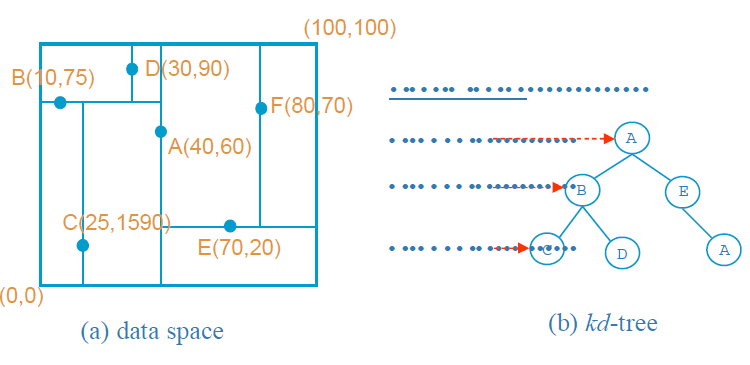
\includegraphics[width=0.5\textwidth]{kdtree}
\caption{kd-tree}
\label{figkdtree}
\end{figure}


When an item is deleted, a node from the sub-tree must be replaced. Here arises a complication that based on the discriminator in that level, let's call it i, either the node with the smallest i in right sub-tree should be replace or  the node with the biggest i in left sub-tree. A non-homogeneous kd-tree was proposed to make this process cheaper. 
Kd-Tree has been used a lot in intensive searches, but some variants has been introduced to make a better performance in clustering, searching, storage efficiency and balancing [survay], such as …..
and below we discuss some of them.

Main memory storage of the index trees are mostly a problem, since it is too big to be placed there  [survay]. Hence, the storage has to be done into disk space. Using binary search tree paging techniques [CeS82 survay] or tree organization of B-trees [BaM72 survay] to store the kd-Tree proposes new indexing structures.

Using properties of both kd-tree and B-tree [reference], the KDB-tree rebuilds the kd-tree to improve some inefficiencies of it.  It means benefits of the balanced kd-trees and the I/O efficiency of B-trees are together. It uses the disk space to bring the kd-tree on disk. 

The method which is used to build  KDB-tree is a space partitioning structure such that the partitions do not overlap each other. The partitions which stand for pages as organizational units, are organized in k-d-tree structure. 
KDB-tree has two basic structures: region page, consist of (region, pageID) pairs, and point page, consist of  (point, pageID) pairs. The region page contains the description of its subpages and a reference to those pages. The point pages contains actual data and references to them. 

\begin{figure}
\centering
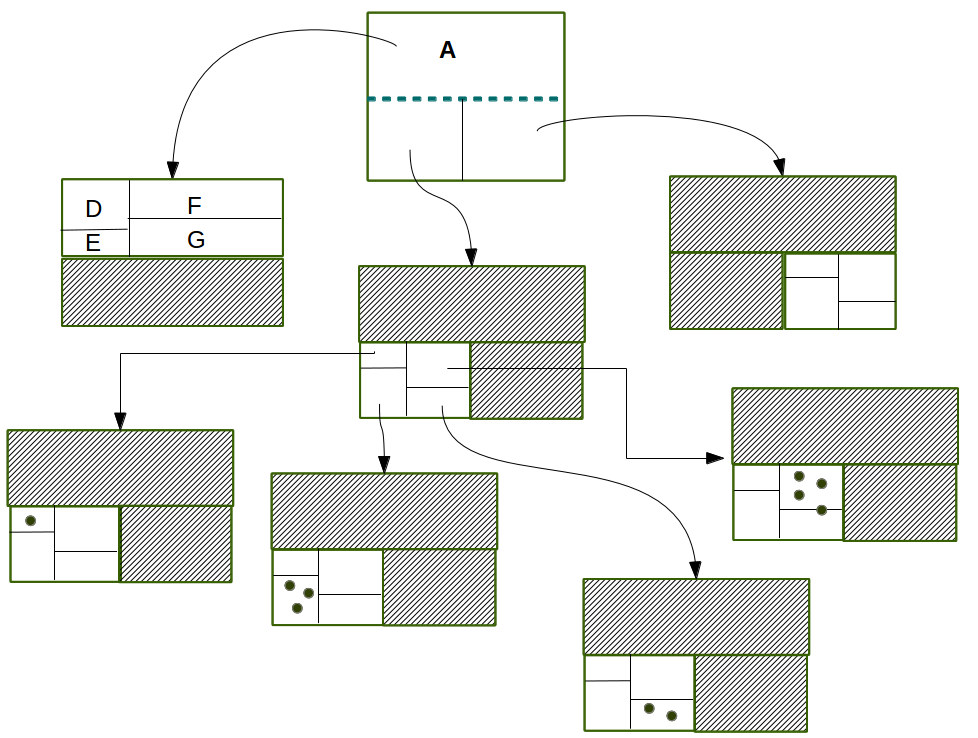
\includegraphics[width=0.5\textwidth]{kdbtree}
\caption{kdb-tree}
\label{figkdbtree}
\end{figure}

The pagination of the B-tree is integrated in the KDB-tree and consequently the tree is height-balanced. Space utilization and efficiency might be low or high, though, since the downward propagation of splitting, caused by region split, may cause low storage utilization. On the other side, there is no guarantee for minimum space utilization. Since partitions do not overlap, it is not always easy to find disjoint partitions to divide a region. So, those partitions must be split at the same value as parent, even though they do not use the minimum amount of space specified for each node. By this problem the range queries' performance is poor. 

Another variation of KDB-Tree which can be distinguished by two features: …
Since in a the region split in lower levels result in sparse nodes, hB-Tree (the holey brick Btree) as a multi-attribute index structure is proposed. Data spaces could be holey. It allows the data space associated with a node to be non-rectangular and it uses kd-trees for space representation in its internal nodes. The leaf nodes are known as data nodes and the internal node as index nodes. An index node data space is a union of its child node subspaces which are obtained through kd-tree recursive partitioning. It is height balanced since it is based on the K-D-B-Tree. 
Advantages of this structure is removing the sparse nodes of the K-D-B-Tree and reduction of search time and space utilization, since kd-tree is used. 
Disadvantages of this structure is that the deletion and splitting of nodes are expensive and also multiple references to a data node will lead to more than one traversal of a path.

\begin{figure}
\centering
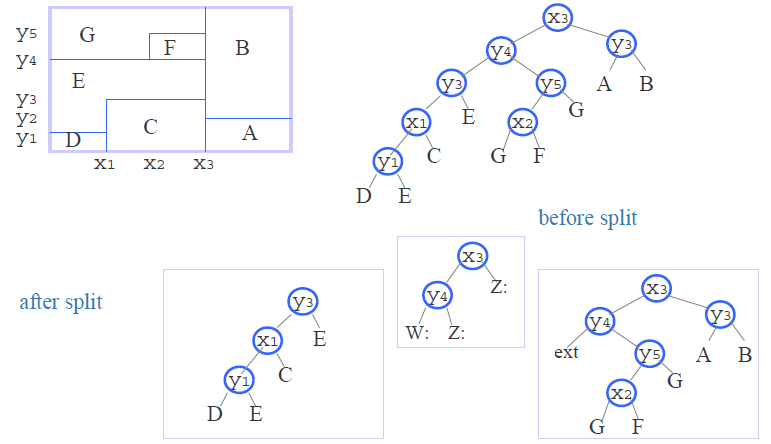
\includegraphics[width=0.5\textwidth]{hbtree}
\caption{hb-tree}
\label{fighbtree}
\end{figure}

\emph{Matsuyama’s kd-Tree}.
This structure is introduced for non-point objects and an extensive duplication strategy is used. The directory is a kd-Tree and a data page is associated for each leaf and those objects which overlaps multiple data spaces are identified in data page and also duplicates. Hence, the data page contains identifiers of the objects totally or partially contained in the corresponding data space.
The point is that this structure is not suitable for large objects since duplication and redundant storage of objects would result in high overhead.

\emph{4D-tree}
Indexes rectangular objects using kd-tree by mapping the objects into points in a four-dimensional space. Each 2D rectangle with (x1, y1) and (x2, y2) is considered as a 4D (x1, y1, x2, y2). As kd-tree the discriminators are choosen cyclically from this set. For each node, a discriminator, discriminator value and pointers to two children are stored. 
For a region search (qx 1, qx 2, qy 1, qy 2), depending on the discriminator, one of the x1 <= qx2, x2  >=  qx1, y1 <= qy2 or y2 >= qy1 has to be done to determine which subtree (or both) has to be searched.
The major problem associated with the 4-d-tree is its intersection search, which can be very costly due to the need for traversal of both subtrees when a query region lies in a subspace that cannot not bounded tightly using the discriminator values.

\emph{skd-tree}
The spatial kd-Tree alters the kd-tree in a way that objects are indexed by their centroid and the minimum bounding box of the object is also stored in the node. This structure is suitable for non-point spatial objects. In a kd-tree the objects which are contained in more than one space, will be referenced more than once. To avoid the duplication virtual subspaces are defined which include the original subspaces. So, each object are placed in the subspace based on its centroid.
With this devision, we just need one more value for each subspace which shows min/max values along the dimension of the discriminator. Therefore, the structure of each node would consist of:
Two children
The discriminator and it's value
The max/ min value of objects left(LOSON)/right(HISON) subspaces along with dimension of the discriminator
The maximum/minimum value of LOSON/HISON the nearest virtual line which bounds the data whose centroid are inside the LOSON/HISON.

\begin{figure}
\centering
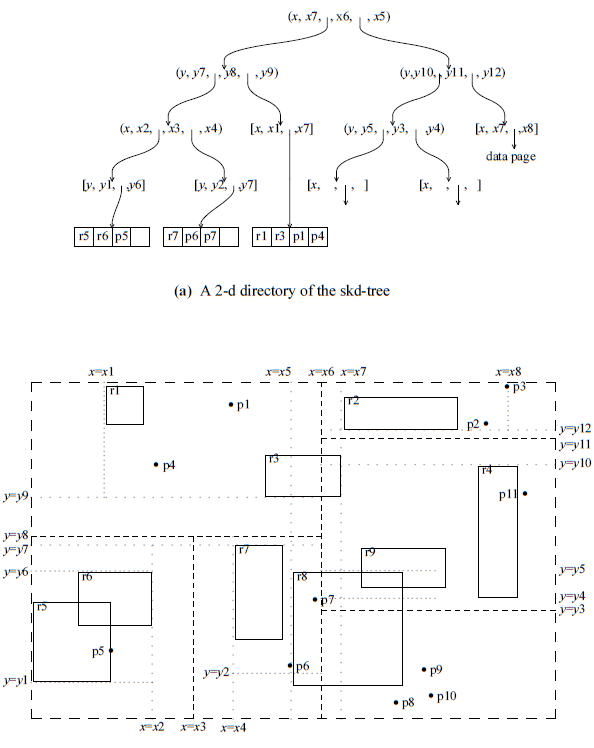
\includegraphics[width=0.6\textwidth]{skdtree}
\caption{skd-tree}
\label{figskdtree}
\end{figure}

During traversal a rectangular space is associated with each node and materialized  such that is tested against the query region if it intersects the region. 
(Since the virtual boundary may sometimes bound the objects tighter than the partitioning line, the intersection search takes advantage of the existing virtual boundary to prune the search space efficiently. To further exploit the virtual boundaries, containment search which retrieves all spatial objects contained in a given query rectangle was proposed. During tree traversal, the algorithm always selects the boundaries that yield smaller search space. The direct support of containment search is useful to operators like within and contain. The search rapidly eliminates all objects that are not totally contained in the query region.)
The Sdk-tree is memory-based, not a disk-based, data structure, thus is not suitable for very large databases.

\subsubsection{B-tree based Indexing Technique}
\emph{R-tree}
\label{rtree}

Minimization of both coverage and overlap is crucial to the performance of R-trees.
\subsubsection{$R^*$-tree}
The $R^*$-tree is found to be more efficient than some other variants, and the R-tree using linear splitting algorithm is substantially less efficient than the one with quadratic splitting algorithm. In general, the R*-tree is an improvement over the R-tree at the expense of more expensive insertion.

This structure tries to reduce overlaps between directory rectangles and the area covered by a rectangle, in order to make better performance, since minimum overlaps leads to less number of branches to be traversed in queries and minimum coverage helps to decide on the paths to traverse on higher levels. 
R*-Tree does these optimizations with revised node split and also forced insertion which finds a better place for a node that its original place. In R-Tree insertion-build structure is highly suboptimal and insertion and deletion could improves the R-Tree dramatically.
 (Using the idea of reinsertion of the R-tree, Beckmann et al proposed a reinsertion algorithm when a node overflows. The reinsertion sorts the entries in decreasing order of the distance between the centroids of the rectangle and the covering rectangle and reinserts the first p (variable for tuning) entries. In some cases, the entries are reinserted back into the same node and hence a split is eventually necessary. The reinsertion will no doubt increase the storage utilization; but it can be fairly expensive when the tree is large. The R*-tree is found to be more efficient than some other variants, and the R-tree using linear splitting algorithm is substantially less efficient than the one with quadratic splitting algorithm. In general, the R*-tree is an improvement over the R-tree at the expense of more expensive insertion.)

\emph{The Buddy Tree}
(In comparison to previously proposed tree structures such as the K-D-B-tree, the buddy-tree guarantees a more efficient dynamic behavior.Moreover, indirect splits which cause low storage utilization and high insertion costs in the K-D-B-tree, are completely avoided. This structure is 
It avoids the downward splitting of the K-DB-tree, the overlapping problem of the R-tree and the dependency of structures upon the insertion of data. The buddy-tree generalizes the buddy system of the grid-file to organize correlated data efficiently, by bounding the data points tightly using the bounding rectangle concepts of the R-tree and organize the directory as in the R-tree. Like grid-files, the non-zero sized data have to be mapped into higher dimension.
An important feature of the buddy-tree is that it does not partition empty data space. Therefore queries, such as partial match queries, where the query region intersects with empty data space, can be performed much faster than by conventional structures partitioning the complete data space.
The following summarizes the design properties of the buddy-tree:
empty data space is not partitioned
insertion and deletion of a record is restricted to
exactly one path
no overflow pages
directory grows linear in the number of records
performance is basicly independent of the sequence of
insertions
efficient behavior for insertions and deletions
very high fan out of the directory nodes)

\emph{The Packed R-Tree}

In order to minimize storage space, coverages and overlaps in R-Tree, constructing a static tree is proposed. To make this tree, first the objects are ordered along a coordinate. The object with the minimum value then is choosen to find the M nearest objects to that one, and assigns them to a node. Here M is the maximum number of objects that are allowed in a page. This step is repeated until the whole objects are assigned to a node. The bounding box of the leaf nodes are higher level objects. These are also ordered and assigned to the nodes. The process repeats until the number of the remained nodes is less than M. If so, they are assigned to the root.
The main objective of the algorithm is to reduce the storage space, the coverage and overlap of rectangles, in order to improve the search efficiency.

\emph{R+-Tree}

This structure is a compromise between the R-tree and the K-D-B-tree, to solve the overlapping problem of covering rectangles. It has just some difference:

Nodes of an R+-tree are not guaranteed to be at least half filled.
 The entries of any intermediate (internal) node do not overlap.
 An object identifier may be stored in more than one leaf node.

The duplication of the objects in the tree avoids overlappings and consequently leads to less path traversals in point queries. 
On the other hand there is some disadvantages: it might be bigger that R-Tree as a result of duplications, and the construction and maintenance are more complex that R-Tree or other variants. 
Also, in insertion cases into the tree a case would happen that the covering rectangles of some entries can prevent each other from expanding to include the new object. In other words, some space ("dead space") within the current node cannot be covered by any of the covering rectangles of the entries in the node. If the new object occupies such a region, it cannot be fully covered by the entries. When a new object cannot be fully covered, one or more of the covering rectangles are split. This means that the split may cause the children of the entries to be split as well, which may further degrade the storage efficiency.
In performance study, in the comparison between R-trees and R+-trees, it is found that the R+-tree requires much more splits, especially for large data objects, but lesser splits for smaller data objects. 
In general, the query efficiency tests show that R+-trees perform better for smaller objects and slightly worse off for larger objects.

\emph{STR-tree}

\emph{Cell-tree}
The cell tree introduces a structure to overcome the overlapping bounding rectangle problems of R-trees and the "dead space" (empty space) problems of R+-trees. Partitioning is done in a recursive way, but not necessarily with rectangles. Instead, the regions are polyhedral, as bounding polygons. Subspaces do not overlap.  
\begin{figure}
\centering
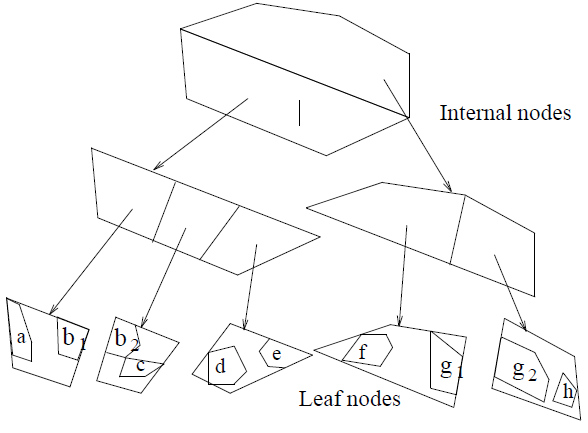
\includegraphics[width=0.5\textwidth]{celltree}
\caption{cell-tree}
\label{figcelltree}
\end{figure}

Like R+-Tree, objects might be represented in more than one leaf node. One problem with such an instruction which duplicates the objects is that each new object may be divided into multiple pieces in order to store them in a tree where internal node bounding polygons do not overlap. Specially in populated DBs. 
(Each split of a node leads to a decrease in the node data space but to an increase in the number of nodes per object. To overcome the fragmentation and duplication problems, Gunther and Noltemeier proposed to store oversized objects which may greatly increase the number of object identifiers being stored in the leaf nodes in separate "oversize shelves". These oversize shelves are data nodes linked to internal nodes in the cell-tree, in one way, causing the tree to be not height-balanced. The placement of a new object in the subtree or oversize shelf requires some optimization. The oversize page shelf can be overflowed and a split on this shelf is necessary.)
\emph{Quadtree}
It is organized in a way similar to the region quad-tree. A region is recursively partitioned until the resulting quadrants do not contain any rectangle. During the subdivision, all rectangles that intersect with either of the two partitioning lines are associated with the partitioning lines. The rectangles that are associated with a quadrant must not belong to any ancestor quadrant. It is assumed that no two rectangles overlap.
\newpage








\section{Related work}
\label{s.rwork}
Here, we are going to summerize a large set of literature over different methods
to store and process GML~\cite{gml} data. Section~\ref{storage} studies
different approaches to store GML. These approaches are investigated
with respect to the effectiveness of storage models in terms of query processing.
After the discussion over storage, the different proposed query languages
will be explained in Section~\ref{queryLang}. Finally, we will look at the
famous databases in Section~\ref{s.dbs} and what they did to handle
GML data.
  
\subsection{Storage}
\label{storage}
One of the basic approaches to store GML data is proposed in \cite{Li2004}.
In this approach, the schema tree is generated at first. Then, the generated
tree is mapped to a relational schema to store all spatial objects as 
values of the mapped tables' field. Spatial query can be submitted 
in XQuery\cite{xquery}-like language with spatial functional extensions.
These GML queries are translated into equivalent SQL queries which are evaluated 
using spatial database management system.

Another similar approach is discussed in \cite{Zhu2011}. Here, GML is stored and queied 
focusing on non-schema documents. After the generation of the GML parse tree,
the nodes are analyzed and schema mapping is generated to store the doc in object-relational DB. 
Both spatial and non-spatial queries are supported in this approach.

Shulian Zhang et al~\cite{Zhang2008} considered both characteristics of XML DB 
and GML spatial data. Here, a native XML database based GML storage is proposed. 
A prototype system is developed on the basics of JAXP (Java API for XML Processing) program API 
and JTS~\cite{jts}, containing schema mapping constructor, document storage tool, 
and spatial analyzer.

\subsection{Query Languages}
\label{queryLang}
XQuery language, recommended by \emph{W3C}, is only 
applicable to non-spatial data. To query spatial data in GML,
Fubao~\cite{Fubao2010} expanded the data model, algebra, functions, operations, 
and formal semantics in XQuery to achieve a GML query processor.
This processor deals with both non-spatial and spatial queries, 
and the results will be outputted in GML.
Supported data types are  Geometry, Coord, Coordinates, Point, LineString, LinearRing, 
Polygon, Box, GeometryCollection, MultiPoint, MultiLineString, and MultiPolygon.
Also, defined spatial operations are simple geometry operation, spatial relation 
operation, spatial analysis operation and specific geometry operation.
The operations are actually handled by JTS in background.

Beside GML is used to represent and exchange 
the geographic data, it also benefits its XML-based model in interoperability, 
and more importantly, could be queried. In \cite{corcoles2001}, the data model 
and algebra behind the language are based on a previously proposed model 
in which components and interrelations are represented as a directed graph. 
The vertices of this graph are geometry types and properties. The edges also
represent the element containment, relationship between elements, and values. 
This query language tries to provide an interface like SQL to work with GML.

Xia Li~\cite{Lisa2006} defines XQuery as a language  not suitable to query GML, 
since spatial related data types and semantics need to be treated different from XML. 
The purpose of this study is to define expand XQuery not for predefined GML elements, 
but more flexible.  A set of operators and functions on GML data types that cover 
the most typical queries over spatial data. The difference with the previous one is 
that this language is applicable not for predefined GML types, but to any type.

Chen~\cite{Chen2010} introduces a new integration of GML and XQuery. In this work,
spatial data types and operations are added to XQuery based on \emph{OGC Simple
Features Spesification} for \emph{SQL} to achieve GML spatial data query.
%Adding spatial data types 
%(Point, LineString, LinerRing, Polygon, MultiPoint, MultiLineString, MultiLinerRing 
%and MultiPolygon) and spatial operation functions (basic, relational, analysis,.. functions), 
%based on OGC Simple Features Specification for SQL, to XQuery can achieve GML spatial data query. 
%Moreover to the previous studies in this subject GML spatial data query language 
%based on XQuery, problem of GML spatial data query, reasons for extending XQuery to
%support GML spatial data query, features of GML spatial data query language, 
%content of XQuery spatial extension, architecture of GXQuery, implementation methods 
%of GXQuery, and query examples of GXQuery were detially studied and discussed. 
The following part of the code shows the idea. 

\begin{verbatim}
FOR $var1 IN doc(“CDUTCampus.gml”)//Building,
$var2 IN doc(“CDUTCampus.gml”)//Building
WHERE $var1/gml:name/node() = “CDUT Palestra”
AND $var2/gml:name/node() = “CDUT Gymnasium”
RETURN geo:Contains(geo:Envelope($var1), $var2)
\end{verbatim}

A semantic version of Xpath language is defined in \cite{Alemdros2011, Alemdros2013}, 
which is not based on the tree-based (syntactic) structure of the GML.
A system based on the semantic structure of GML is developed to store GML by PostGIS RDMS.
Then, Xpath queries are translated into SQL language, considering the GML schema
and the resulted query is represented in KML \cite{kml} in this system.

\cite{Gutierrez2004} A knowledge-based approach is used to querying heterogeneous spatial databases based on an ontology and conceptual and attribute similarities. The ontology, which may be independent of the databases, expands and filters a user query. Then, queries are translated into a formal specification of entity classes, which are compared against definitions in databases. This process is carried out by determining the conceptual similarity between entities in a user ontology and by comparing these entities in the ontology with entities in the conceptual models of databases. In addition, the specification of a query is done not only by identifying entity classes but also by considering constraints based on attribute values.

\cite{corcoles2004} Towards integrating spatial and non-spatial data, it's necessary to develop an integration sys. For querying the data in different sources. Here a prototype of a mediation system for querying XML spatial resources in GML is studied.  The main task of this approach is to provide users with a unique interface for querying spatial XML resources with different schemas, independently of their organization and location. It provides the infrastructure for formulating structured spatial queries by taking into consideration the conceptual representation of a specific domain in the form of an ontology. The resources are integrated using RDF. The most novel and critical feature of this approach is the querying of spatial XML resources, because it uses a different way from that of querying and relating non-spatial resources.

\cite{belussi2006} Base on the problem posed in different representation of spatial data in various resources ( For example, one dataset M1 may represent roads and bridges as regions, another dataset M2 may represent roads as regions and bridges as lines, a third dataset M3 may represent both as lines), or even in integration scenarios or architectures, a possible solution is to introduce some mechanism of query relaxation, by which approximated answers are returned to the user. In this study, the relaxation problem for spatial topological queries is considered. In particular,  some relaxed topological predicates are presented and is show in which application contexts they can be significantly used. In order to make such predicates effectively usable, the way that GQuery, an XML-based spatial query language, can be extended to support similarity-based queries through the proposed operators is also discussed.

\begin{verbatim}
Determine all roads overlapping some bridge.
for $x in document(bridge.xml), $y in document(road.xml)
where overlap($x/geometry, $y/geometry) = true
return $x

Determine all roads overlapping some bridge, up to a 22% error.
for $x in document(bridge.xml), $y in document(road.xml)
where overlap($x/geometry, $y/geometry,R,L,0.22) = true
return $x 
\end{verbatim}

Finally, a novel approach is propsed by Corcoles~\cite{corcoles2003} to integrate Geospatial data on the Web.
This data is stored and queried using GML format and a special query language. 
An ontology is used to solve the semantic heterogeneity of different GML documents.

\subsection{Geospatial Data in Well-known Databases} ??
\label{s.dbs}
Besides analysing some ideas in the field of geospatial processing in databases, 
it would be useful to see the geospatial features and functionalities in similar database systems 
In this section, geospetial issues in three well-known databases, MongoDB, eXist, MarkLogic 
are explained to see how the different ideas are being provided and being used in practice. These database are 
selected since they are new in this filed and also all having geospatial functionalities. 


\subsubsection{MongoDB}
\label{mongo}
\cite{mongogeneral2010}
\cite{mongoinaction2011}

Geospatial Index:

There is two special indexes in MongoDB: 2d indexes that uses planar geometry when returning results and 2sphere indexes that use spherical geometry to return results.

When an index is created, geohash values for coordinate pairs are calculated and then the geohashes are indexed.
Geohash is calculated by recursively dividing the a 2D map into quadrants and assigning each area a 2-bit value.


If the file contains just flat data, the 2d Index has to be used, but for those which also contain spherical data, 2sphere Index has to be choosen, since the distance function differs respectively.

Later on geohash values will be index using B-Tree. 
MongoDB also used B-Tree structure for other type of index, such as Single Field (e.g. indexing over names), Compound, Text Index. (Probably this point effect on the structure of geospatial index.)

Geospatial Functions:

geoWhithin, near (flat space), nearSphere (spherical space), geoIntersect, which could be mixed with other non-spatial functions (like find, ...). 
centerSphere (for spherical space), center (for flat space, define a circle with a specified radius), maxDistance (mixed with near functions to specify the demanded distance), box (defines a box, could be also mixed with geowithin function), polygon (defindes a polygon), inqueDocs (to prevent a through put a document twice in query results)

\begin{figure}
\centering
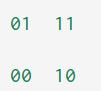
\includegraphics[width=0.1\textwidth]{mongoformat}
\caption{MongoDB Format}
\label{fig}
\end{figure}

mongoformat

Geohash (wikipedia)
Geohashes offer properties like arbitrary precision and the possibility of gradually removing characters from the end of the code to reduce its size (and gradually lose precision).
As a consequence of the gradual precision degradation, nearby places will often (but not always) present similar prefixes. Conversely, the longer a shared prefix is, the closer the two places are.
The main usages of Geohashes are
as a unique identifier.
represent point data e.g. in databases.
When used in a database, the structure of geohashed data has two advantages. First, data indexed by geohash will have all points for a given rectangular area in contiguous slices (the number of slices depends on the precision required and the presence of geohash "fault lines"). This is especially useful in database systems where queries on a single index are much easier or faster than multiple-index queries. Second, this index structure can be used for a quick-and-dirty proximity search - the closest points are often among the closest geohashes.
One limitation of the Geohash algorithm is in attempting to utilize it to find points in proximity to each other based on a common prefix. Edge case locations close to each other but on opposite sides of the Equator or a meridian can result in Geohash codes with no common prefix.[1]
Secondly a geohash essentially defines a bounding box within which a location lies, therefore two locations may be spatially very close but have different geohashes. In order to be useful to proximity searches, the surrounding eight geohashes of a geohash must be calculated and the locations matching these pulled out, therefore complicating potential usage in proximity searches.

\subsubsection{MarkLogic}
Geospatial data is marked up in XML elements and/or attributes. MarkLogic could handle and query different formats, such as GML, KML, GeoRss, and even general format for geometric data which are not based on a specified format. Only WGS84 and Raw coordinate systems are supported. WGS84 is used for data on the earth geometry, and raw coordinate system is suitable for data on flat plane.

Regarding the geospatial queries, the following types are supported:
\begin{itemize}
\item point query--matches a single point
\item box query--any point within a rectangular box
\item radius query--any point within a specified distance around a point
\item polygon query--any point within a specified n-sided polygon
\end{itemize}

Additionally, there are some Geospatial Operations as built-in functions to perform operations on geospatial data (in cts namepsace):

 box-intersects → Returns true if the box intersects with a region.
 circle-intersects → Returns true if the circle intersects with a region.
 polygon-intersects → Returns true if the polygon intersects with a region.
 complex-polygon-intersects → Returns true if the complex-polygon intersects with a region.
 polygon-contains → Returns true if the polygon contains a region.
 complex-polygon-contains → Returns true if the complex-polygon contains a region.
 distance → Returns the distance (in miles) between two points.
 shortest-distance → Returns the great circle distance (in miles) between a point and an region. The region is defined by a region.
 destination → Returns the point at the given distance (in miles) along the given bearing (in radians) from the starting point.


 XQuery Primitive Types And Constructors
These constructors (as functions from search module, cts namespace) are used in geospatial queries (cts:query constructors), defining regions as instances of cts:region, then the query returns true if the searching data are inside the region.
 cts:box 
 cts:circle
 cts:complex-polygon
 cts:linestring
 cts:point
 cts:polygon

 WKT

	WKT language also is supported for geospatial data representation. The parse-wkt function is used when WKT is used. It converts WKT to sequence of region items. Also, cts:to-wkt function could convert cts:region type in MarkLogic to WKT.

GeoSpatial Coordinates and Regions in MarkLogic Server


Latitudes and longitude pairs shape point. Points shape other geometries, like circle or polygon. Boxes are formed by 4 points which on the surface of the Earth, the edges of the box are arcs, but when those arcs are projected into a plane, they become two-dimensional latitude and longitude lines, and the space defined by those lines forms a rectangle.


The Geospatial Index
It is not based on quad or R-tree. It works like a range index with points as data values. In this range index, every value is a pair of latitude and longitude. Like an array of x,y values, sorted mainly based on lat and then long values. The values in array also are connected to the corresponding doc.
The points would be founded easily in a sorted structure. Boxes could be found first by finding the lat range, then checking for the long range. For circles and polygon as more complex ones, the bounding box is used to find the region they belong to. Also, to check if a point is inside the polygon, the number of intersections with the northward or southward arc of the point is counted. 

…. 

Different types of Geospatial Indexes: (???)

 Geospatial Element Indexes: data is represented by whitespace or punctuation separated element content 
 Geospatial Element Child Indexes: data comes from whitespace or punctuation separated element content, but only for elements that are a specific child of a specific element.
 Geospatial Element Pair Indexes: data comes from a specific pair of elements that are a child of another specific element.
 Geospatial Attribute Pair Indexes: data comes from a pair of specific attributes of a specific element.
 Geospatial Path Range Indexes: data is expressed in the same manner as a geospatial element index and the element or attribute index is defined by a path expression.


Geospatial Index Positions
	For each geispatial index there is a positions options, which is used for queries with restrictions of data distance inside the document.

Geospatial Lexicons1
Provided by spatial index, containing unique values of  geospatial data. 

“geo” XQuery Library
geo:box
Create a cts:point value from an element representing a box in one of the supported markup vocabularies.
geo:circle
Create a cts:circle value from a radius and an element representing a point in one of the supported markup vocabularies.
geo:geospatial-query
Returns a cts:query matching points within given regions.
geo:geospatial-query-from-elements
Returns a cts:query matching points within given regions.
geo:interior-polygon
Create a sequence of cts:polygon values from a polygon element in one of the supported markup vocabularies.
geo:point
Create a cts:point value from an element representing a point in one of the supported markup vocabularies.
geo:polygon
Create a cts:polygon value from a sequence of point elements in one of the supported markup vocabularies.


“gml” XQuery Library
gml:box
Create a cts:box value from a GML Envelope element.
gml:circle
Create a cts:circle value from a radius and GML Point element.
gml:geospatial-query
Returns a cts:query matching points within given regions.
gml:geospatial-query-from-elements
Returns a cts:query matching points within given regions.
gml:interior-polygon
Create a sequence of cts:polygon values from a GML Polygon element.
gml:point
Create a cts:point value from a GML Point element.
gml:polygon
Create a cts:polygon value from a sequence of GML Point elements or a GML Polygon element.


“geoRss” XQuery Library
georss:circle
Create a cts:circle value from a radius and GeoRSS point element.
georss:geospatial-query
Returns a cts:query matching points within given regions.
georss:point
Create a cts:point value from a GeoRSS point element.

“kml” XQuery Library
kml:box
Create a cts:point value from a KML LatLongBox element.
kml:circle
Create a cts:circle value from a radius and KML Point or Location element.
kml:geospatial-query
Returns a cts:query matching points within given regions.
kml:geospatial-query-from-elements
Returns a cts:query matching points within given regions.
kml:interior-polygon
Create a sequence of cts:polygon values from a KML Polygon element.
kml:point
Create a cts:point value from a KML Point or Location element.
kml:polygon
Create a cts:polygon value from a KML polygon or a sequence of KML Point or Location elements.


“cts” Functions
Part of these functions also contain geospatial function: 1 2
----------------------------------------------------------------------------------------------------------------------------
For querying on geospatial data, after loading the data into the DB and making the indexes, primitive types should be constructed to be used in the geospatial cts:query functions. Then, geospatial queries needs to be constructed, using primitive types. 
Also, there are modules to convert the Metacarta, GML, KML, and GeoRSS formats to cts:box, cts:circle, cts:point, and cts:polygon formats, to pass them into the cts:query constructors and make appropriate queries.

\subsubsection{eXist-db}
The design if spatial index in eXist-db doesn't store character data from the document. It stores WKB index entries in a JDBC database, namely a HSQLDB. In other words, the spatial data is stored in the DB, but geometries, as JTS Geometry instances, are held in memory, waiting for a special mode to be flushed into a relational DB, insertion or removal. The Geometry WKT would be serialized and deserialized to and from the database.
The index is made by the relational db (uses an SQL database to index spatial data) and the geometric functions are applied using JTS library.



Both PostGIS and Oracle Spatial share the same “R-Tree” [1] spatial index structure. R-Trees break up data into rectangles, and sub-rectangles, and sub-sub rectangles, etc. It is a self-tuning index structure that automatically handles variable data density and object size.

Ideas

Query general format geospatial data, considering the data as a set of points, ...
Storing the eospatial data in geohash ???
…


\subsection{Others}
\newpage

















\section{Spatial Querying in BaseX}
\label{s.basex}
%TODO tozihe bishtar dar more requirements va inke chera injuri develop shode
%TODO:why gml:http://www.w3.org/Mobile/posdep/GMLIntroduction.html - 
%TODO: and  http://spatialnews.geocomm.com/features/gml/topten.html
Spatial query is a spacial type of query which requires the processing of geometries with two certain properties in general. First, it has geometries as inputs and outputs as well as other primitive types, like double, integer, etc. Second, it considers spatial relations between the geometries.
As we discussed in Section~\ref{s.dbs}, there are various viewpoints in providing geospatial features in a database to fulfill the expected requirements. Following the OGC Simple Feature (OGCSF)~\cite{springergeo} data model, geospatial features in BaseX adapt the EXPath geospatial API function interface specification which defines commonly used functions from the OGCSF Common Access API \cite{simpleFeature}. Since the OCGSF data model is typically represented in GML, we concentrate to add the support of GML format in BaseX. However, an implementation would support the other encodings, like KML. 

Throughout the following sections, we discuss the integration of geospatial data processing in BaseX. We introduce geospatial functions as a new module, called \textit{Geo Module}, in Section~\ref{geomodule}. Query efficiency is improved later in Section~\ref{indexBX} by implementing an index structure. Indexing and the related time complexities are discussed hereafter in Section~\ref{indexFunc} and Section~\ref{BXevaluation}, as the critical issue in this topic. Finally the concluding is explained in Section~\ref{BXconc}.

\subsection{Geo Module}
\label{geomodule}
As mentioned above, geospatial features in BaseX are implemented based on the EXPath Geo Module Specification \cite{expath}. This specification contains the definition of functions for widely used geographic and geometric analysis operations, from OGCSF Common Access API version 1.2. These functions apply to geometries in different formats, such as GML, KML, GeoJSON, Well Known Text (WKT), and even Well Known Binary (WKB). Based on the specification, Geo Module in BaseX comprises a set of functions, such as intersection, within, distance, boundary, centroid, diference, union, and etc., added to the \textit{basex-api} package. The geometries supported in this module are Point, LineString, Polygon, MultiPoint, MultiLineString, and MultiPolygon. This module is an individual package with a set of classes as briefly described below,
\begin{itemize}
\item \textit{Geo}: This class is the main class, in which all geo spatial functions are defined. The set of functions in this class include those which are used in XQuery. The complete list of functions and their description are available in the online BaseX documentation.
\item \textit{GeoError}: This class defines error functions with related massages which are thrown when an error occurs.
\item \textit{GeoTest}: Test functions for the \textit{Geo} class are implemented here.
\item \textit{GmlReader}: Functions required to parse GML geometries as XML elements, are implemented in this class.
\item \textit{GeoIndex}: Besides, this class implements the functions related to the geospatial index. 
\end{itemize}

Geospatial index structure is implemented in BaseX core. Spatial indexing and related implementation details will be described in Section~\ref{indexBX}. Here, we explain general functionalities of this module.

The geospatial functions, defined as public methods in \textit{Geo} class, are accessible from BaseX GUI. They use some private methods to read geometries or write them out into the GUI. Besides, each function employs the corresponding function from the JTS library to do the required geometric operation and to provide the appropriate result. Here, we shortly explain the process by which the input geometries, either from a variable or a database node, are processed.


Suppose we are searching for all geometries within a specified polygon ($\$p$). The query should be written using XQuery via BaseX GUI as follows,
\vspace{10px}
\begin{fakeJSON}
let $p := 
<gml:Polygon>
  <gml:outerBoundaryIs> ... </gml:outerBoundaryIs>
</gml:Polygon>
for $x in //gml:Polygon
  return if ( within($x, $p) ) then $x else ()
\end{fakeJSON}
\vspace{10px}
Each geospatial function has at least one geometry as input, like the above \textit{within} function. In this example, the $\$p$ variable is provided as a docment node and the $\$x$ variable iterates all Polygon nodes in the current database. Various function are involved in processing this query. Followings, this process which is illustrated in Figure~\ref{figGeoModuleProcess} is explained in detail. 

To read the geometries as a document node, the private function \textit{geo} makes sure that the node name is at least a valid geometry name. It means if the element name is something out of the set of geometry names, the function will throw an error. 
Then, the GmlReader class is used to read and parse the whole element and to check the validity based on GML 2.0 format. Regarding the JTS limitation, geometries have to be in GML 2.0 format to be validated and analyzed for further operations. 

The forementioned GmlReader class reads the elements differently based on their types, i.e., tag names. If the element is a valid GML geometry, the function creates the corresponding geometry, using JTS constructors. Otherwise, the matching error massage will be shown. For instance, if a polygon does not have any outer ring or if the coordinates of a ring do not shape a closed ring, an error will be thrown. 

 \begin{figure}
\centering
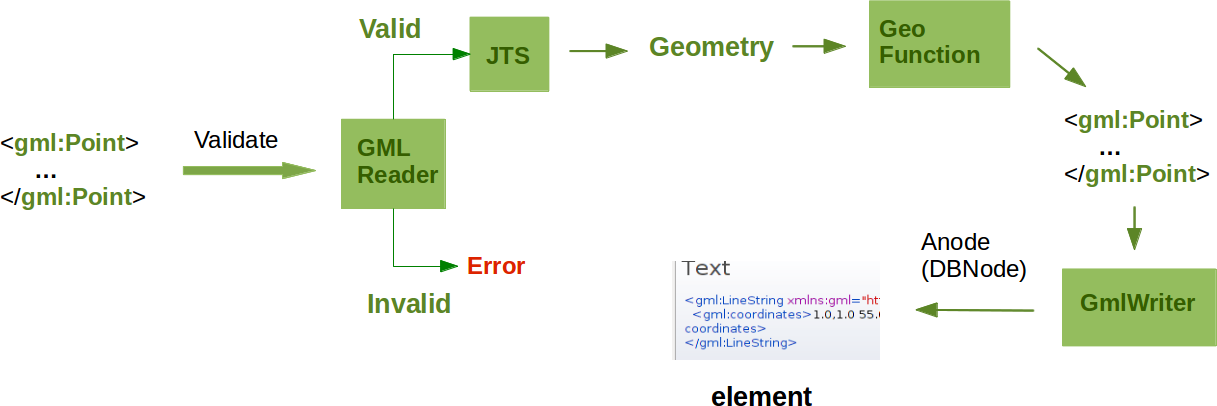
\includegraphics[width=0.95\textwidth]{GeoModuleProcess}
\caption{Converting GML elements to geometris}
\label{figGeoModuleProcess}
\end{figure}

Now, the geometries are ready to be processed in a geometric operation, like checking two geometries whether they intersect each other, finding the symmetric distance of two geometries, or getting the number of inner rings of a polygon. The operations are done using the JTS functions. The output could be in any XML Schema (XSD) data types, such as integer, boolean, string, URI, and etc., or GML 2.0 Geometry. The XSD type are equivalet to the BaseX defined data types. That means primitve data types like boolan, integer, and string are represented in BaseX as \textit{Bln}, \textit{Str}, and \textit{Int} classes respectively. The Geometry type, which can be the output of functions like the intersection, union, and difference of two geometries, must be returned as an element in the abstract node (\textit{ANode}) type to be in compliance with the specification. Having the output geometries in GML format, GMLWriter function converts them first to a string, using JTS GmlWriter and builds a database node (DBNode) hereafter. Considering the point that DBNode extends the ANode class, the output node is sent to the GUI and is shown as a gml element, expressing the geometric result. 

Although the geo functions are working, the query performance seems not satisfying. Having commonly huge geospatial data, performance problem is serious. The common solution is an indexing algorithm designed to improve the efficiency. Since the geospatial data is a written form of geometries positioned in the space, an indexing structure can be designed considering the positions. In the following sections, we discuss an indexing approach and its influce on performance in comparison with the no-index querying.


\subsection{Geospatial Index in BaseX}
\label{indexBX}
To enhance the geospatial query time in BaseX, we discuss an index structure. This index avoids processing the whole database when partial checking of the file would be enough. For this purpose, a bounding box is computed for each geometry by which an efficient filtering can be applied. For example, if we want to find the objects within a specific geometry, examining just the area near to this geometry is adequate. If two geometries have intersecting bounding boxes, they might intersect each other and have to be checked weather they fulfill the query condition. Otherwise, they will not have any contact and there is no need to check them. This approach decreases the number of scanned geometries and consequently gives the better timing, which we call it two step filtering. The two step filtering is clarified as followings,
\begin{enumerate}
\item Finding the geometries which their bounding box intersect with the bounding box of query area
\item Checking the selected geometries against the query condition
\end{enumerate}
%Moreover, functions of this module in which a big number of geometries from the database coule be involved, have the time complexity bigger than O(1) and need a spatial indexing to be handled in shorter time. %TODO conintinue


 \begin{figure}
\centering
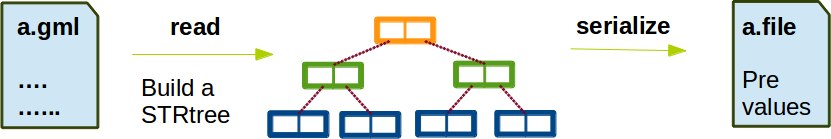
\includegraphics[width=0.95\textwidth]{IndexinFile}
\caption{Geospatial index creation}
\label{figIndexinFile}
\end{figure}


Among the spatial index structures discussed in Section~\ref{geospatialindex}, JTS supports the STRTree and QuadTree. Davis~\cite{jts-presentation} discussed that STRTree in contrast with QuadTree can not be updated after the generation. However, we choose the STRTree since it has better performance. As mentioned before, STRTree has the basic of R-Tree with the improved performance. The index tree structure, holding the bounding boxes in inner nodes and geometries in leaves, is made once when the spatial index for the database is requested and written into a file on disk. This process is illustrated in Figure~\ref{figIndexinFile}. Each time the index is demanded, the file is read into the main memory and the two step filltering is executed. It should be mentioned that only the following queries would benefit from this index. The definitions of these functions are provided in EXPath Geo Module specification.
\begin{itemize}
\item intersects (geometry1, geometry2)
\item within (geometry1, geometry2)
\item contains (geometry1, geometry2)
\item overlaps (geometry1, geometry2)
\item crosses (geometry1, geometry2)
\item touches (geometry1, geometry2)
\end{itemize}

The spatial index is involed both in BaseX core and \textit{basex-api} packages. The main structure of the index is added as a package in core, called \textit{index.spatial}. This package contains the index builder classes based on the core index structure of BaseX. The class \textit{SpatialBuilder} which extends \textit{IndexBuilder}, builds the index tree using pre-values instead of the tag names to address the database elements. Then, JTS serializer writes the tree structure into a file called \textit{STRTreeIndex}.

The other GeoIndex class in \textit{basex-api} package extends \textit{QueryModule} class and implements the method defined by JTS STRTree class for reading the index file from hard disk into memory. Additionally, this class implements the \textit{filter} method to do the first step of two step filtering. The datails of the index implementation is described in the following section.
 
\subsection{Index Functions Implementation}
\label{indexFunc}
To add the spatial index, we tought of two approaches. The first approach implements new signature for the forementioned functions in a new class. It means the index filter function is encoded directly in the existing geo functions. Then queries can be done with the new spatial function as in Code~\ref{intersectIndx}.
\vspace{10px}
\begin{fakeXML}[label=intersectIndx,caption=The geo function containing the index functions]
import module namespace geo-index = "http://expath.org/ns/GeoIndex";
let $a:= <gml:Polygon> ... </gml:Polygon>
return geo-index:intersects("DB", $a) 
\end{fakeXML}

\vspace{10px}
\begin{fakeXML}[label=geoandfilter,caption=Geo function used with index function]
import module namespace geo-index = "http://expath.org/ns/GeoIndex";
import module namespace geo = "http://expath.org/ns/Geo";
declare namespace gml="http://www.opengis.net/gml";
let $a:= <gml:Polygon>
                <gml:outerBoundaryIs>
                  <gml:LinearRing>
              	    <gml:coordinates>
              	      3.9,50.6 6,52.8 4.5,52.8 3.9,50.6
              	    </gml:coordinates>
                  </gml:LinearRing>
                </gml:outerBoundaryIs>
             </gml:Polygon>
return ( geo-index:filter("DB", $a)[geo:intersects( $a, .)])
\end{fakeXML}
\vspace{10px}

Since having two functions with the same name and functionality is redundant, we introduce a new approache in which the \textit{filter} function can be used in XQuery to benefit from the index stucture. In this way, a sample query would be as in Code~\ref{geoandfilter}. To summerize these approaches, the former approach as in Code~\ref{intersectIndx}, does the whole process including the fisrt step of filtering through the \textit{geo-index:intersects} function, while the latter approach as in Code~\ref{geoandfilter}, uses the original \textit{geo:intersects} function together with \textit{geo-index:filter} which does the first step of filtering. 


The negetaive point about the latter approach is that the input polygon, like polygon $\$a$ in Code~\ref{geoandfilter}, is read, parsed, and created every time that the spatial function, here \textit{intersects}, is called in the \textit{for} loop, evevn though it is the same fixed object. Since, this causes redundancy and consumes a considerable amount of time, we use a map to hash the fixed input and prevet the further redundant reading. This will dramatically reduce the query time, as shown in Figure~\ref{figMap}.
 \begin{figure}
\centering
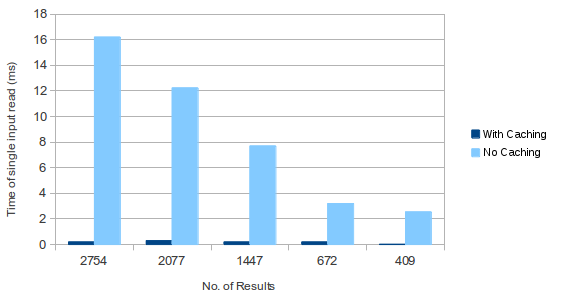
\includegraphics[width=0.9\textwidth]{MapIndexing}
\caption{Using a Map to cash the input geometry: performance effect}
\label{figMap}
\end{figure}

Figure~\ref{figMap} demonstartes the time consumed by different queries to read the single input geometry with or without cashing. It could be seen that when no map is used, as the number of results goes higher more time is taken, while by cashing the time consumption remains constant, since the input geometry is read once. In other words, the input geometry will be read each time the function \textit{geo:intersects} is called without cashing, as it is one of the input arguments. In the next section, we assess the performance isues related to the geoapaial index.

\subsection{Evaluation and Improvement}
\label{BXevaluation}
%TODO:jomle aval beravad b sectione ghabl
There is no need to emphasize on the importance of the role that indexing plays in the query time and the performance improvement. Here, we use real-world data to observe the effect of the currently implemented spatial index, followed by in depth looking at the implementation from other perspectives. The aim is to find ways in order to improve the performance. This data is provided by University of Twente, Department of Geoinformation Processing and holds some real information on the Earth in GML 2.0 format. The original file is based on one of the Netherlands coordinate system (RD/NAP Amersfoort RD New) and is around $133.3$ MB including the $12773$ polygons inside the $11886$ multipolygons.
We run different queries on this database with and without geospatial index to see time consumption dependency on the index structure. 
\begin{figure}
\centering
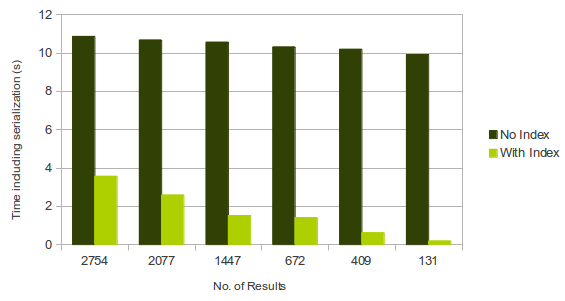
\includegraphics[width=0.85\textwidth]{IndexEfficiency}
\caption{Query performance improvement by using geospatial index}
\label{figIndexEfficiency}
\end{figure}

Since queries have various number of results, we can see the trend changes in regards to the number of outputs.
To start with, we take a look at the effect on index utilization in queries in comparison with queries using no spatial index. Figure~\ref{figIndexEfficiency} represents the effectiveness of index utilization.
As shown in Figure~\ref{figIndexEfficiency}, when geospatial index is not used, the query time remains constant for every query regardless of the number of results. As we discussed in Section~\ref{indexBX}, this is because of the fact that for each query, the whole file is scanned and analyzed. In contrast, queries using geospatial index relatively take more time as the number of output objects goes higher. It confirms that filtering approach are going in the right direction, but the performance still is not satisfying. Thus, we need to investigate more ways to improve it.
\begin{figure}
\centering
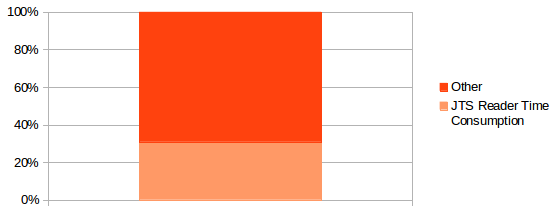
\includegraphics[width=0.8\textwidth]{JTSReadetTimeConsumption}
\caption{JTSReader time consumpion in total query ime}
\label{figJTSReaderTime}
\end{figure}
By monitoring the times consumed by different part of a query, we discovered that JTS GMLReader functions takes considerable amount of time (see Figure~\ref{figJTSReaderTime}). This time is taken by \textit{JTS GMLReader} class by which the geometries are read from GML and converted to \textit{JTS} geometries. 

\begin{figure}
\centering
\subfigure[Through JTS GMLReader]{
	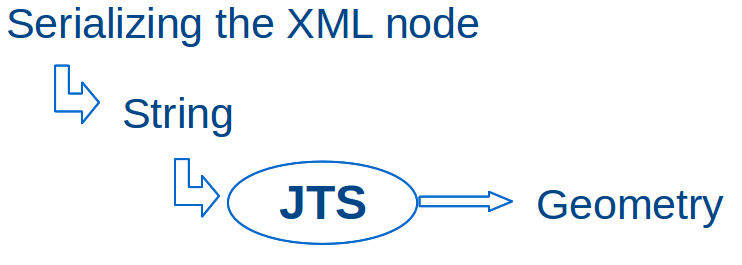
\includegraphics[width=0.47\textwidth]{GmlReaderProcess1.png}
	\label{figParseProcess1}
}
\centering
\subfigure[Through Custom GML Reader]{
	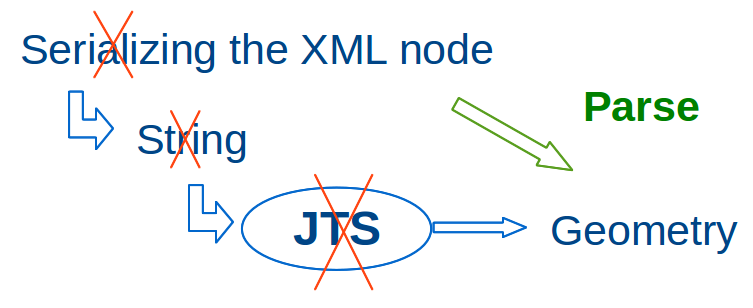
\includegraphics[width=0.47\textwidth]{GmlReaderProcess.png}
	\label{figParseProcess2}
	
}
\caption{Parsing process of the GML elements}
\label{figParseProcess}
\end{figure}

Regarding the geometry reading process by JTS, shown in Figure~\ref{figParseProcess1}, it seems that the direct parsing approach might decline the query time. Thus, we implement a custome GML reader class to immediately parse the GML elements into the JTS geometries (see Figure~\ref{figParseProcess2}). To assess the time efficiency, a set of queries are tested and the results are presented in Figure~\ref{figGmlReader}. 

\begin{figure}
\centering
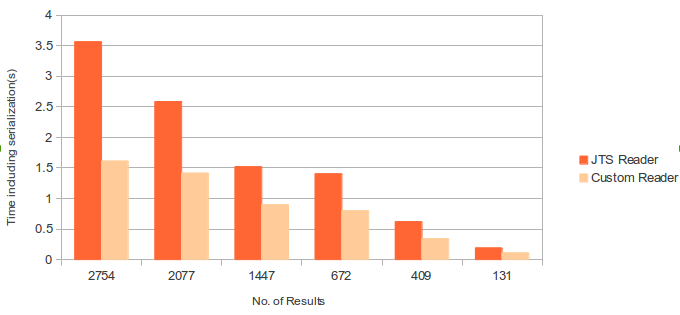
\includegraphics[width=0.8\textwidth]{GmlReader}
\caption{Custom GMLReader vs. JTS GMLReaer}
\label{figGmlReader}
\end{figure}

As it was supposed, reading time drastically reduced by using the new reader functions, although both have increasing trend proportional to the number of outputs.%gosaste

A deeper look at the different parts of a query will be beneficial to find the parts where need to be concentrated more in order to achieve better performance. Suppose we run the query below,
\vspace{10px}
\begin{fakeJSON}
let $a:= <gml:Polygon> ... </gml:Polygon>
return ( geo-index:filter("DB", $a) [geo:intersects( . , $a)]).
\end{fakeJSON}
\vspace{10px}
The total query time will be divided into the following parts,

\begin{enumerate}
\item reading the input geometry \textit{\$a}
\item filtering the geometries using \textit{filter} function by pre values 
\item reading the filtered geometries from the database using selected pre values
\item apply \textit{intersects} operation on the pair of input geometry and each selected geometries.
\end{enumerate}

To see how each part influence the performance, we examine them separately. Figure~\ref{figDetailedTiming} shows the times taken by the above-mentioned actions. It could be seen that the biggest amount of time is spended reading the geometries. Even the single reading of the input geometry seems to be expensive. Hence, the reading function should be observed more in detail.

\begin{figure}
\centering
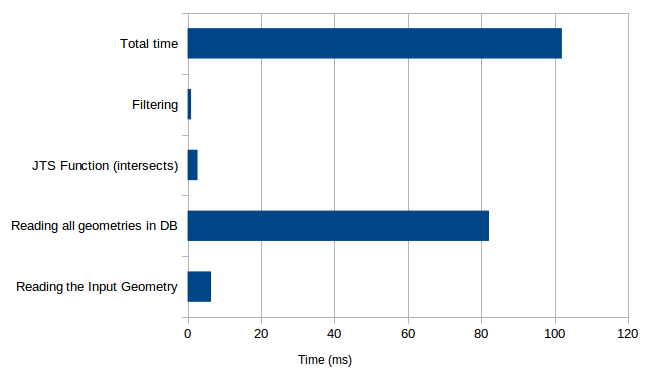
\includegraphics[width=0.8\textwidth,height=0.25\textheight]{detailedTiming}
\caption{Detailed timing in a query using geospatial index}
\label{figDetailedTiming}
\end{figure}


We have used Java profiling to get more precise information. The first few methods in profile output with the highest percentage of time occupation, ordered from the most-used to the least-used, are listed in the following,

\vspace{10px}
\begin{tabular}{l l l c l}
\textbf{rank} & \textbf{self} & \textbf{accum} & \textbf{count} & \textbf{method} \\
 & & & &\\
1 & 6.95\% & 6.95\% & 94 & org.basex.util.Token.{\color{red}split}\\
2 & 5.33\% & 12.28\% & 72 & org.expath.ns.GmlReader.createPolygon \\
3 & 4.59\% & 16.86\% & 62 & org.basex.util.Token.{\color{red}split} \\
4 & 4.22\% & 21.08\% & 57 & org.basex.query.func.JavaModuleFunc.eval \\
5 & 3.55\% & 24.63\% & 48 & org.expath.ns.Geo.geo \\
6 & 3.18\% & 27.81\% & 43 & org.basex.util.Token.{\color{red}split} \\
7 & 3.03\% & 30.84\% & 41 & org.basex.util.Token.{\color{red}split} \\
8 & 2.96\% & 33.80\% & 40 & org.basex.util.Token.{\color{red}split} \\
9 & 2.74\% & 36.54\% & 37 & org.expath.ns.Geo.geo \\
\end{tabular}
\vspace{10px}

As the profile output indicates, the \textit{split} function calls consume the greatest amount of time. Besides, \textit{createPolygon} and \textit{geo} functions, all used in \textit{GmlReader} class, are expensive. Therefore, these functions should be focused in performance tuning. 
\begin{figure}
\centering
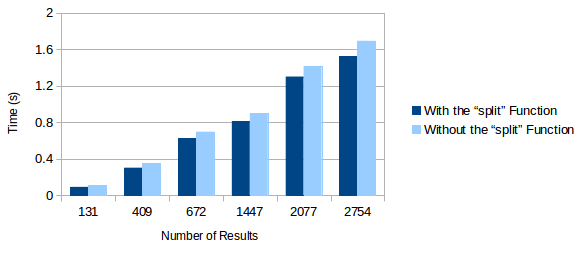
\includegraphics[width=0.8\textwidth,height=0.2\textheight]{BXSplit}
\caption{The query times of the selected queries before and after the removing of \textit{split} function}
\label{figBXSplit}
\end{figure}
Since the \textit{split} function has the most frequent call, we discard it in favour of better performance. This function is used to divide a "coordinate" string regarding the delimiters to make coordinate pairs. We replaced it with a piece of code to parse this string. 
A "coordinate" value in GML 2.0 can include different points which are separated with a space. Each point in the coordinate of GML 2.0 have two dimensions $X$ and $Y$ seprated with a comma. Code~\ref{coord-example} shows an example of the GML 2.0 coordinate. Based on this format, the new code reads the "coordinate" string and acts based on the position and type of delimiters and numbers. Therefore, the coordinate pairs are constructed from a valid string. Otherwise, an error massage will be shown. Figure~\ref{figBXSplit} shows the effect of removing the \textit{split} function on the query times. As can be seen in this Figure, this effect grows as the number of results gets bigger.
 
\vspace{10px}
\begin{fakeXML}[label=coord-example,caption=An example of GML 2.0 coordinate]
<gml:coordinates>
  3.9,50.6 6,52.8 4.5,52.8 3.9,50.6
</gml:coordinates>
\end{fakeXML}
\vspace{10px}

In addition to the \textit{split} function, we omit the $Z$ values in parsing process, since the $Z$ value is ignored with the geospatial function. It means it is useless to read this $Z$ value. It can be considered as a limitation of GML 2.0 which is improved in GML 3.0. Not surprisingly, excluding the $Z$ values from the parsing process declines the query time that is displayed in Figure~\ref{figBXZvalue}. This effect is minor in the smaller number of results and is more obvious with more output numbers.

\begin{figure}
\centering
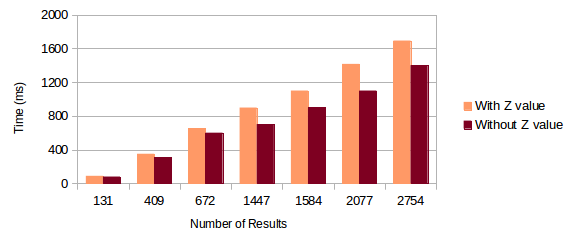
\includegraphics[width=0.8\textwidth,height=0.2\textheight]{BXZvalue}
\caption{The effect of ignoring the $Z$ values of coorinates in GML parsing on query times}
\label{figBXZvalue}
\end{figure}

Up to this point we have tried various ways to decrease the query times in Geo Module. Further attemps could be done following the feorementioned Java profiling list, if the implementation will be continued in the current direction.

\subsection{Conclusion}
\label{BXconc}
In this Section, we discussed the Geo Module implementation details and assessment in BaseX which provides a set of geometric functions based on the EXPath Geo Module specification. This module employs the JTS library to compute the geometric operations. To enhance the performance, the JTS STRTree index structure is added that accelerates the execution time of queries such as intersects, within, inside, and touches. This is done by applying a filtering in the STRTree structure and consequently reducing the number of processes in the database. Besides the index tree, a GML Reader class is developed to parse the gml elements directly regarding the inefficieny in JTS GMLReader. Although the timing results are convincing, there are room for improvements. For example, the function \textit{split}, \textit{geo}, and \textit{createPolygon} can be modifiend in favour of better performance.

\newpage
\section{BaseX vs MongoDB}
\label{s.mongo}
%TODO:Complete

An introduction of MongoDB geospatial features is provided before in \ref{mongo}. In this section, we will have a more-detailed overview of these functionalities and a comparison between BaseX and MongoDB. However these two systems follow distinct approaches, it would be beneficial to review MongoDB as a rather new, recently developed, and widely used database system. MongoDB is among the few NOSQL systems providing geospatial features. Here, we will mainly see differences between these systems, particularly in performance of the same features. This comparision empowers us to improve the geospatial querying performance in BaseX. 

As we discussed in Section~\ref{mongo}, geospatial data can be represented in MongoDB either as planar or spherical maps. Since the earth is a spherical globe, the geospatial calculations on planar maps are only an approximation~\cite{coordsys,coordsys-mongo}. As an example, the measurement of distances in planar maps are accurate only in a small region. It means the spherical maps are the better representation when the calculations are expected as real ones on the Earth. As our goal is to assess some geospatial features of MongoDB and compare it with Basex Geo Module, we focus only on the spherical approach. Correspondingly, WGS84 is used instead of legacy coordinate pairs to express the spherical maps. 

\vspace{10px}
\begin{fakeXML}[label=feature-collection,caption=A GeoJSON file containing a \textit{FeatureCollection} object]
{
  "type": "FeatureCollection",
  "features": [
    {
      "type": "Feature",
      "geometry": {
        "type": "Point",
        "coordinates": [102.0, 0.5]
      },
      "properties": {
        "prop0": "value0"
      }
    },
    {
      "type": "Feature",
      "geometry": {
        "type": "LineString",
        "coordinates": [
          [102.0, 0.0], [103.0, 1.0], [104.0, 0.0], [105.0, 1.0]
        ]
      },
      "properties": {
        "prop1": 0.0,
        "prop0": "value0"
      }
    }
  ]
}
\end{fakeXML}
\vspace{10px}


Geospatial operators of MongoDB for spherical data support the GeoJSON~\cite{www/geojson} format. GeoJSON is a human-readable encoding format for representing the geographical features, using JSON standard. It consists of an object which describes a geometry, Feature, or collection of Features. The type of geometries must be one of these types: Point, LineString, Polygon, MultiPoint, MultiLineString, MultiPolygon, and GeometryCollection. A \textit{Feature} must have members with the names \textit{geometry} and \textit{properties}. A feature collection is an object with the type \textit{FeatureCollection} which must have a member with the name \textit{features}. Code~\ref{feature-collection} is an instance GeoJSON file with a \textit{FeatureCollection} object.

Current version of MongoDB supports only three geometry types Point, LineString, and Polygon. As mentioned in Section~\ref{mongo}, a geospatial query in MongoDB can use \textit{geoIntersects}, \textit{geoWithin}, \textit{near}, and \textit{nearSphere} operators. In addition, there are geometry specifiers to define geometries in query conditions of these operators. For instance, the \textit{\$center} and \textit{\$centerSphere} are specifiers for a circle area in planar and spherical maps on which the user intends to do the query. Then, the user can find all geometries within a determined circular area. Another example is the \textit{\$maxDistance} specifier that determines the maxmimum distance from a point in order to find geometries within this particular distance. Geometry specifires are limited to, \textit{\$geometry}, \textit{\$maxDistance}, \textit{\$center}, \textit{\$centerSphere}, \textit{\$box}, and \textit{\$polygon}. An example demonstrating the usage of the specifiers in a query is provided in the followings,
\vspace{10px}
\begin{fakeJSON}
db.<collection>.find( { <location field> :
                         { $geoWithin :
                           { $centerSphere :
                              [ [ <x>, <y> ] , <radius> ] }
                      } } )
\end{fakeJSON}
 \vspace{10px}
 
In the following sections we will compare these two databases regarding the query performance. 
In Section~\ref{s.query}, we analyze specific test queries. Then, the assessment continues
utilizing the indexing structure in Section~\ref{index}. Later, the update functionality of databases is 
investigated in Section~\ref{update}. Finally, Section~\ref{conc} contains the conclusion and further work.

\subsection{Querying the Databases}
\label{s.query}
To analyse and compare the databases behaviour, designing the same test queries on the identical dataset is the most straight-forward approach. Based on the MongoDB geospatial features and properties, the Netherland test dataset must be changed. A brief explanation of the changes is provided here to clarify the rules and limitaions. The main change was to either remove multipolygon from the dataset or transforming them to a set of distinct polygons, since multipolygon is not supported in this version of MongoDB. Besides, the coordinate system is converted to WGS84. At the end, there are 12773 polygons and no multipolygon in the data file. Since the geometries are changed in database and the results would be different, we repeate all queries with the new dataset in BaseX.

To start with, the GeoJSON file containing the geometries, is imported into MongoDB. This can be done  using Java API or Mongo Shell with appropriate \textit{mongoimport} command. There are limitations to consider in importing the GeoJSON in MongoDB. The main one is the \textit{document} size limitation in a \textit{collection}. Document and collection are two concepts in MongoDB which are correspond with a table and a record in this table respectively. A collection can have one or more documents and a document is a set of key-values. A database contains one or more collections. To successfully import a document into a collection, it should be smaller than 16MB. Since it is common to have large geometries in real-world geographic data files, this limitation can be a problem. Aother limitation is that the $z$ coordinate is not supported in MongoDB. When a coordinate contains $z$ dimension, although those geometries are not processed, no error massage is shown during the import process and query. MultiPoint, MultiLineString, and MultiPolygon, which are not supported in MongoDB, are also skipped in queries without any error massage. 

The above-mentioned size limitation made us to change the file structure again.
When the file structure was in the form of Code~\ref{feature-collection}, 
an error message regarding the size limitation was thrown. 
When the GeoJSON file structure is changed to contain individual features as below,
this problem disappeared.
\vspace{10px}
\begin{fakeXML}[label=features,caption=A GeoJSON file restructured regarding the size limitation]
    {
      "type": "Feature",
      "geometry": {...},
      "properties": {...}
    },
    {
      "type": "Feature",
      "geometry": {...},
      "properties": {...}
    }, 
    { ... }, ..., { ... }
\end{fakeXML}
\vspace{10px}
%TODO:explain about the query difficulties and aggregation of the above structure
After importing the file, we examined the common features, i.e., intersection, within, 
functionalities in both databases.
%and near  
The queries in Code~\ref{basex-query} and Code~\ref{mongo-query} find the intersecting geometries from the Netherland's dataset with the given polygon in BaseX and MongoDB. The polygon coordinates are determined for different queries in the following way. At first, the maximum and minimum coordinates are found in the dataset. After that, we generate differet input polygons in regard to these boundaries. The polygons coordinate are altered such that the number of results differes in each query.
\vspace{10px}
\begin{fakeXML}[label=basex-query,caption=Example query of \textit{intersects} function in BaseX]
import module namespace geo = "http://expath.org/ns/Geo";
declare namespace gml="http://www.opengis.net/gml";
let $a:= <gml:Polygon>
              <gml:outerBoundaryIs>
                <gml:LinearRing>
                  <gml:coordinates>
                    6,52.6 6.1,52.6 6.1,53 6,53 6,52.6
                  </gml:coordinates>
                </gml:LinearRing>
              </gml:outerBoundaryIs>
            </gml:Polygon>
for $b in //gml:Polygon 
return if (geo:intersects( $a, $b)) then $b else ()
\end{fakeXML}
\begin{fakeXML}[label=mongo-query,caption=Example query of \textit{intersects} function in MongoDB]
db.places.find( { geometry :
                  { $geoIntersects :
                    { $geometry :
                      { type : "Polygon" ,
                        coordinates:[[[6,52.6],[6.1,52.6],
                        	    [6.1,53],[6,53],[6,52.6]]]
                } } } } )
\end{fakeXML}
\vspace{10px}

Similar queries are designed to check the other functions. Here, we skip the queries and directly go to the results. To check the profiling in MongoDB, query plan information, such as the index type, the query time, scanned objects, etc, \textit{\$explain} operator could be specified either in the forms,
\vspace{10px}
\begin{fakeJSON}
db.collection.find()._addSpecial( "$explain", 1 )
db.collection.find( { $query: {}, $explain: 1 } )
\end{fakeJSON}
 or 
 \begin{fakeJSON}
db.collection.find().explain().
 \end{fakeJSON}
\vspace{10px}
Below the profile of a sample query is shown,
\vspace{10px}
\begin{fakeJSON}
"cursor" : "BasicCursor",
"isMultiKey" : false,
"n" : 2756,
"nscannedObjects" : 12773,
"nscanned" : 12773,
...
"millis" : 43907,
...
"server" : "MongoServer"
\end{fakeJSON}
\vspace{10px}

In the provided information, number of the results and the query time is implied in \textit{n} and \textit{millis} elements respectively. \textit{cursor} specifies the type of the cursor used by the operation. Here, \textit{BasicCursor} indicates that the query is only performing a normal scan to find the results.  This typical cursor reads the documents in natural order. That is, no index is used for this operation and the whole data is scanned in the original order. If a geospatial index is used, the cursor type will change. The value\textit{n} reflects the number of geometries that match the query condition, i.e., the number of items on the cursor. \textit{nscanned} is the number of scanned documents for this operation, when no index is used, or scanned index entry in the range, when an index is used. \textit{nscannedObjects} is the number of scanned documents in this query to obtain the results. In queries which an index structure is not used, as in the above sample, these two numbers will be equal. Otherwise, \textit{nscannedObjects} may be lower, as shown in the following query plan which uses a geospatial index. 
In other words, $nscanned\geq nscannedObjects\geq n$ always. Ofcourse, the most optimum state is where $nscanned=nscannedObjects=n$. 
\vspace{10px}
\begin{fakeJSON}
...,
"cursor" : "S2Cursor",
"isMultiKey" : true,
"n" : 2756,
"nscannedObjects" : 3370,
"nscanned" : 36941,
...,
\end{fakeJSON}
\vspace{10px}

%and it could be reached with compound indexes and rephrasing the query statement in some cases as well.
%TODO mesal for optimization from: http://Java.dzone.com/articles/optimizing-mongodb-compound

Running the same queries as before, like \textit{intersects}, in both databases, Figure~\ref{figBXvsMongoNoIndexIntersects} shows the timing of various queries without using any geospatial index. As it could be seen, all query times are more or less the same, since the whole data is scanned when no index is used. It is also obvious from the following query plan in MongoDB which specifies the cursor type, number of index keys scanned (nscsnned), and number of documents scanned to get the result (nscsnnedObjects),
\begin{fakeJSON}
...
"n" : 12773,
"nscannedObjects" : 12773,
"nscanned" : 12773,
...
\end{fakeJSON}

\begin{figure}
\centering
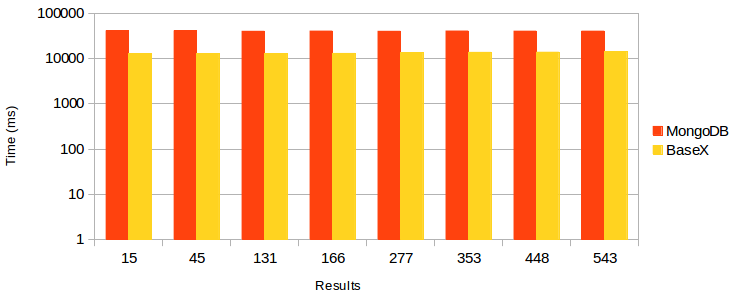
\includegraphics[width=0.8\textwidth,height=0.25\textheight]{BXvsMongo-NoIndex-Intersects-log}
\caption{Query timing of \textit{intersect} operation without geospatial index}
\label{figBXvsMongoNoIndexIntersects}
\end{figure}


Until now, the sample queries are applied to the databases without using any index. 
In the following section, we measure the running time again by applying the geospatial index.
In this way, we also cover \textit{near} and \textit{nearSphere} queries in MongoDB that definately need the geospatial index.  
%using the \textit{distance} function to find the near geometries in BaseX in which the current index structure is not applicable.


%%%%%%%%%%%%%%%%%%%%%%%%%%%%%%%%%%%%%%
%%%% Section: Indexing in the Databases
%%%%%%%%%%%%%%%%%%%%%%%%%%%%%%%%%%%%%%
\subsection{Indexing in the Databases}
\label{index}
The assessment process is continued by applying the geospatial index. In MongoDB there are two choices for using geospatial index, \textit{2d} for data expressed in legacy coordinate pairs and \textit{2dsphere} for both GeoJSON data objects and legacy coordinate pairs. We use \textit{2dsphere} which fits to the choice of sherical maps, via the following shell command,
\vspace{10px}
\begin{fakeJSON}
db.Collection.ensureIndex({geometry:"2dsphere"}) 
\end{fakeJSON}
\vspace{10px}
The same step is also taken in BaseX. Running again the same queries using a geospatial index, supposedly gives declined query times (see Figure~\ref{figBXvsMongoIndexIntersects}). As explained in Section~\ref{s.basex}, index is apllied through the \textit{filter} function in BaseX, while MongoDB follows another approach. MongoDB applies the index in casual query formats after executing the above-mentioned command and there is no need to change the queries in general. 


\begin{figure}
\centering
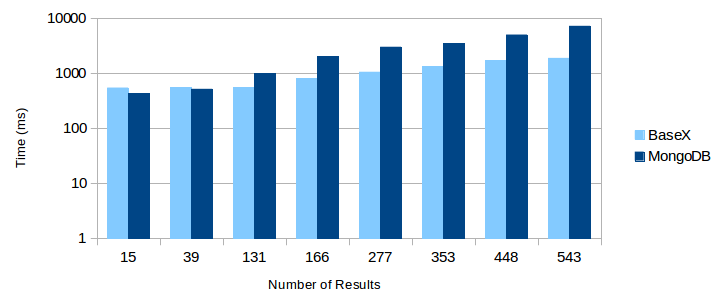
\includegraphics[width=0.8\textwidth]{BXvsMongo-Intersects-Index-log}
\caption{Query timing of \textit{intersect} operation with geospatial index}
\label{figBXvsMongoIndexIntersects}
\end{figure}

%Besides, the search for the geometries within an input area is done in the same way and the timings are shown in Figure~\ref{figBXvsMongoIndexWithin}. It can be seen that the queries with smaller number ofreturned geometries have better performane in MongoDB. Although it seems a positive point to return the big numbers of result in as shorter time as possible, considering smaller returned numbers of results is of greate importance for us, since these queries are more common in real-world usecases.

% TODO
%\begin{figure}
%\centering
%\includegraphics[width=0.7\textwidth]{BXvsMongo-Within-Index}
%\caption{Query timing of \textit{intersect} operation with geospatial index}
%\label{figBXvsMongoIndexIntersects}
%\end{figure}

The next widely used type of query is finding the near places or geometries up to a distance from a specific point. It could be also expressed as finding the geometries inside a circle with the distance value as the radius lenght. This feature is provided in MongoDB via \textit{\$near} and \textit{\$nearSphere} operators which simply get the reference point and the disance and hereafter returns the whole geometries in the specified distance from the point. Both near operators need a geospatial index, either \textit{2d} or \textit{2dsphere}. A specific distance in meter is defined as a condition to filter those geometries within this area. Below, we provide a sample query of the \textit{\$nearSphere} oprator.  
\vspace{10px}
\begin{fakeJSON}
db.collection.find({{geometry:
                       {$nearSphere:
                         {$geometry:
                           {type:"Point", coordinates:[4.5,51.95]}, 
                             $maxDistance : 100
                    }}}})
\end{fakeJSON}
\vspace{10px}
%TODO:reference for projected coordinate sys.
BaseX Geo Module currently provides this feature via \textit{distance} or combination of \textit{buffer} and \textit{within} functions. In Both cases, if the coordinate system in which the data is provided is a projected coordinate system, the distance can be specified in meter or any other metric unit. In a projected coordinate system, all the areas, lengths, and angels are defined on a flat two-dimensional space. In such a system, the user is provided with this \textit{near} feature in BaseX by using the above-mentioned functions as belows,
\vspace{10px}
\begin{fakeJSON}
import module namespace geo = "http://expath.org/ns/Geo";
declare namespace gml="http://www.opengis.net/gml";
let $a:= <gml:Point>
              <gml:coordinates>
               4.5,51.95 
               </gml:coordinates>
            </gml:Point>
for $b in //gml:Polygon 
return if (geo:distance( $a, $b) le 500) then $b else ()
\end{fakeJSON}
\vspace{10px}


For the data provided in a geographic coordinate system, calculations do not work with the metric values. A geographic coordinate system, such as WGS84, defines the areas and locations in a three-dimensional spherical space. Since there is not a specific unit for the current Geo Module functions, the \textit{distance} function interprets the input distance in the coordinate system of the data. For example, our sample Netherlands dataset is in a metric coordinate system. Hence,  the distance value in queries can be specified in meters. %TODO:better description

\begin{figure}
\centering
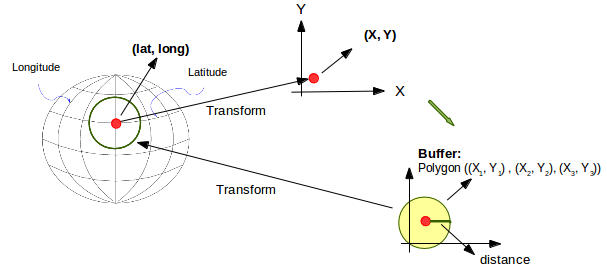
\includegraphics[width=\textwidth]{Transform}
\caption{Having the \textit{near} feature for WGS84 data using transformation in BaseX}
\label{figTransform}
\end{figure}

The forementioned \textit{near} feature as a common use case is available in BaseX only for metric coordinate systems. To provide this feature also for geographic systems via the current geo functions, we need to convert the geographic coordinates to metric ones. In this way, we convert the specified input geometry in WGS84 to a metric system. Then, we compute the buffer of converted geometry up to the input distance in the same metric system and convert the buffer back to the original geographic coordinate system. A buffer of geometry is an identified region within a specific distance of the geometry. At the end, we find the all geometries within the buffer in geographic coorsinate system. This approach benefits from the geospatial index structure, via the \textit{within} function, while the approach with the \textit{distance} function do not utilize the geospaial index. This process is illustrated in Figure~\ref{figTransform}. 
This procedure is expressed as below, using the \textit{buffer} and \textit{within} functions and should return the same result as the previous query, 

\vspace{10px}
\begin{fakeJSON} 
within(geometry,
       transform(buffer(
                   transform(myPoint_in_wgs84, other_metric_cs)
                   , 500)
                 , wgs84
                )
      )
\end{fakeJSON}
\vspace{10px}
Having the same use cases, we have tested this feature in both databases, with the timing result shown in Figure~\ref{figBXvsMongoNear}. BaseX uses the distance function, while \textit{\$nearSphere} operator finds the geometries in MongoDB. Obviously, MongoDB has a better performance, specifically with smaller number of results. The qurey times and the number of results are directly proportional in MongoDB, since index is used and both chaneges accompany each other. BaseX do not use the geospatial index and consequently returns every results more or less in the same time.

%TODO: figure for converion method in BX
%TODO:change the chart for new queries of distance in BaseX


\begin{figure}
\centering
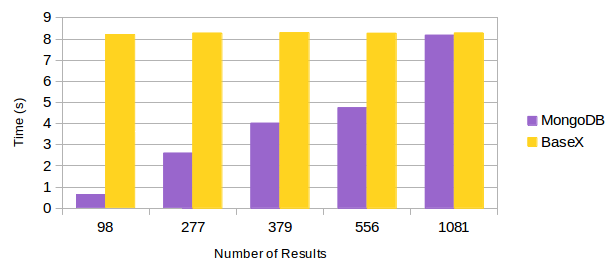
\includegraphics[width=0.8\textwidth]{BXvsMongoNear.png}
\caption{Query timing of the \textit{near} feature}
\label{figBXvsMongoNear}
\end{figure}


As mentioned in Section~\ref{indexBX}, BaseX records the index structure in a file and reads it back into the main memory, when the geospatial index is required. A Point which we should contemplate is to include the time for index opening in query times, since in memory management, the index file might be removed from the memory and read back again. This time is not counted in the presented charts.
%TODO: better explanation


\subsection{Database Update}
\label{update}
%TODO:Complete!not good :|
Updating a database as a significant interaction supplied by the database system generally comprises three different operation: insert, delete, and modify. In addition to the whole issues related to the database update on disk and memory management, reconstructing the indexes is of great importance. That is, since the index is constructed based on the old database state, the updated database needs a new index. 

Currently in BaseX, updating is not applied to the geospatial index after the database update operations. It means the STRTree do not get updated automatically and the geospatial index has to be rebuilt manually. It causes redundant constructions and consequently worse performance. Here, we see how it could effect the updating performance in comparison with MongoDB which manages to rebuild the index in the updating process.

Considering the manual update of the geospatial index in BaseX, reindexing time must be examined to evaluate the updating process. This implies the index creation time plus reopeneing the index file into the main memory should be included in the evaluation. 
As shown in Figure~\ref{figBXvsMongoUpdate}, performance of all update operations in MongoDB are apparantly better. As mentioned before, reindexing in BaseX causes a huge growth in time, which individually takes the greatest amount of total time (See Figure~\ref{figBXUpdate}). We skip the result of deletion and insertion since they follow the similar pattern as update.

The unsatisfactory performance of the updating and also \textit{near} feature in BaseX lead us to a new approach to use the MongoDB index from BaseX. The strategy is explained in the next section.

%TODO this is some part that we can speak about it in Conclusion
%Since the current index implementation do not involves updating based on the STRTree definition, hence a new index should be designed and implemented.................
 


\begin{figure}
\centering
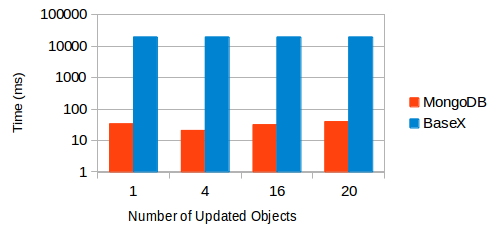
\includegraphics[width=0.7\textwidth]{BXvsMongo-Update.png}
\caption{Performance of the update operation in BaseX and MongoDB}
\label{figBXvsMongoUpdate}
\end{figure}


\begin{figure}
\centering
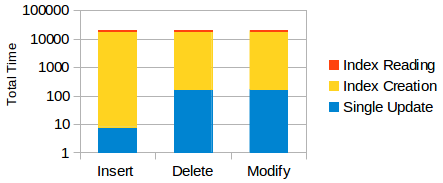
\includegraphics[width=0.7\textwidth]{BXUpdate.png}
\caption{Time consumtion percentage of the update operations in BaseX.}
\label{figBXUpdate}
\end{figure}

\subsection{Querying by MongoDB via BaseX}
\label{MongoviaBX}
Up to this point we have investigated both BaseX and MongoDB to gain some improvement ideas for BaseX. We go further in this way by querying the data with MongoDB through BaseX. A conceivable goal for this approach could be supplying the missing features or make the features with better performance in MongoDB accessible from BaseX. In this approach, BaseX could be used as a coonector to MongoDB, then the provided queries in MongoDB syntax are executed by MongoDB and the results are shown through BaseX. For the missing feature, this would add a functionality to BaseX. But, for the common queries we should evaluate the new query times to see how the performance changes. 
The test implementation is done by defining a connection string and the intended query in a function. However, these tasks could be specified through the XQuery by user and we just have done it as a test. 
In regards to the unsatisfactory query times in the \textit{near} feature, we have tried the \textit{\$nearSphere} operator. The performance modification of this feature is demonstrated in Figure~\ref{figMongoviaBX-near}.
 
\begin{figure}
\centering
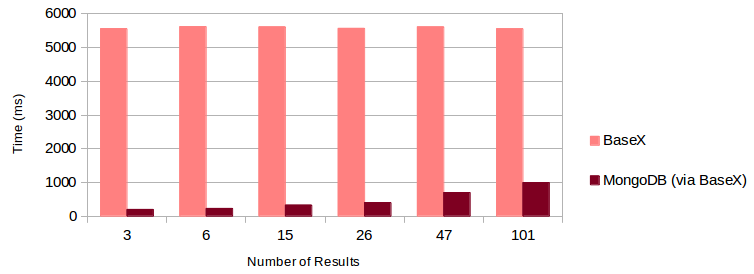
\includegraphics[width=0.9\textwidth]{MongoviaBX-near.png}
\caption{Performance comparision of the \textit{near} feature in BaseX vs. MongoDB through BaseX}
\label{figMongoviaBX-near}
\end{figure}

Figure~\ref{figMongoviaBX-near} implies that the performance of the \textit{near} query executed by MongoDB is preferable. The constant performance trend in BaseX is because of the no index inclusion. Hence, the user can benefit from this functionality in MongoDB through BaseX. 


\begin{figure}
\centering
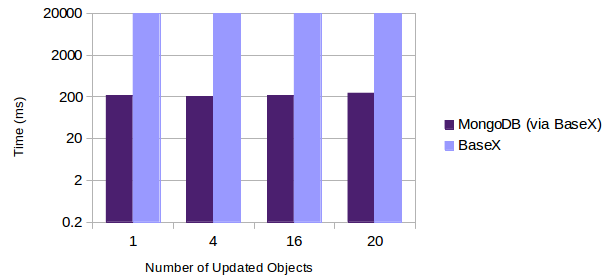
\includegraphics[width=0.8\textwidth]{MongoviaBX-Update.png}
\caption{Performance comparision of the update operation in BaseX vs. MongoDB through BaseX}
\label{figMongoviaBX-update}
\end{figure}

This process is done for the update operaions such that the update query modifies the database in MongoDB. Correspondingly, it should be decided to continue the querying either in MongoDB or in BaseX after repeating the update queries and rebuilding the index structure. Figure~\ref{figMongoviaBX-update} indicates the better timing result of updating by MongoDB through BaseX. 

\subsection{Discussion}
\label{s.disc}
Throughout this section we investigated two strategies to efficiently process the geospatial data in BaseX. Based on these investigations, here we will discuss the  previously-mentioned approaches of the geospatial processing in BaseX and cover the pros and cons of the available approaches, particularly the most recent one in Section~\ref{MongoviaBX}. 

To start with, we suppose that a user has a geospatial dataset in GML and they would like to work in this format in BaseX, since their general requirements are met by BaseX. Based on our examinations, there are some queries in which BaseX is not able to cover them or can not provide some features in a proper timing. It means those cases either are not covered, like updating the index structure or are covered with an apparently poor performance in comparision with the other similar query times, such as the \textit{near} feature. Therefore, geospatial queries such as \textit{intersects} or \textit{within}, can be applied efficiently while some other like \textit{near} and update, can not. Furthermore, regarding to our assumption, some funtionalities of BaseX convinces the user to work with GML. We call them \textit{GML-related} features. We consider these co-called \textit{GML-related} features in our discussion, as they might influnce the geospatial processing approch that wil be preferred.

%Although BaseX can handle the non-geospatial queries as well as some geospatial queries like intersects %and within almost efficiently using Index, the near query and the database update decreases the efficiency dramatically. Therefore, besides the geospatial queries there might be some non-geospatial queries as well, e.g. finding the point elements or the number of polygons in a dataset. It means the geospatial queries are not necessarily the only focuse of the queries and the user can mix both types in a piece of code. Hence, these so-called non-geospatial queries should be considered in the set of user requiremets, however analysing them are not our focuse. This point is important when the user wants to choose between BaseX and MongoDB for geospatial queries while the non-geospaial queries will be done by BaseX. In this case the user can benefi from both databases while the most requirements are fulfilled by BaseX. 

%To summerize the results of our investigations, the near query and the geospatial index updating in BaseX are far from the ......???, though geospatial query times which are the focuse of the index structure, like intersects, seem that could be satisfying in some cases/some how.???  

Table~\ref{t.comparisonBaseXMongo} summerizes the statement above. \textit{MongoDB through BaseX} in this table means BaseX connects to MongoDB to benefit by the features which are not available or available with poor performance in BaseX, as discussed in Section~\ref{MongoviaBX}. \textit{GML-related} features points the forementioned features which are supposed here to be satisfying enough for the user, indicatd with the notation $"\times"$. This assumption is made in order to concentrate on the evaluation of those cases in which the user choose to use BaseX and we try to cover the missing geospatial features.
%Otherwise, the user might choose to work with another system, like MongoDB.
% is better in efficiency.
With $"\times\times"$, we mean that option is very efficient.
\vspace{10px}
\begin{table}
\centering
\begin{tabular}{|l | c | c|}\hline
\textbf{Tasks} & \textbf{BaseX} & \textbf{MongoDB through BaseX}\\\hline
 \textit{GML-related} Queries & $\times$ &\\\hline
 Geospatial Queries,  & $\times$ &\\
like \textit{intersects/within} & & \\\hline
 The \textit{near} Query & &$\times\times$ \\\hline
 DB Update Queries & &$\times\times$ 
%like update/insert/delete &&
\\\hline
\end{tabular}
\caption{The comparison of two strategies; using BaseX or connect to MongoDB via BaseX}
\label{t.comparisonBaseXMongo}
\end{table}
\vspace{10px}

As is expressed in Table~\ref{t.comparisonBaseXMongo}, the geospatial queries like \textit{intersects} and \textit{within} are working with an acceptable performance in BaseX. On the other hand, for the \textit{near} and update queries connecting to MongoDB seems to be the appropriate approach. Hence, a fast conclusion would be to have the advantage of using MongoDB through BaseX. However, the synchronization of the database instace in BaseX and the database instance in MongoDB should be precisely examined. If the user intends to modify the database which means also the modification of index without any further querying regarding the changes, the faster strategy is to update the MongoDB instace, while the database instance in BaseX remains untouched. But, in case that the user wants to do further querying based on the changes, this approach is not optimized.  

One way to discard the above-mentioned problem could be limiting the user to do all geospatial queries regarding the index in MongoDB and use BaseX just as a connector. 
However, as we see in Table~\ref{t.comparisonBaseXMongo} doing some queries in BaseX are more efficient and connecting to MongoDB might be a disadvantage, since this adds at least the connection time to the query time. Moreover, the complete dependency of BaseX on MongoDB for all geospatial queries would be too much and disadvantageous while each system is designed for different requirements and follow various goals. 
%a big limitation for this software regarding the geospatial processing. 
Thus, it will be more appropriate to provide the user with both possiblities.

Table~\ref{t.possibilities} summerizes the sample scenarios that could happen based on the existing features to process the geospatial data. In addition, this table shows the relevant/appropriate actions the user can apply as an efficient strategy toward her/his goal.


\begin{table}
\centering
\scalebox{1}{
\begin{tabular}{|l | l | }\hline
\textbf{Scenarios} & \textbf{What to do?}\\\hline
 Needs a \textit{instersects/within} query  & Using BaseX only\\
and no update and no \textit{near} query  & \\\hline
 Needs a \textit{near} query and no update & Using BaseX and MongoDB together\\\hline
 Needs modifications in the database & Using MongoDB only\\\hline
\end{tabular} }
\caption{Possible scenarios and appropriate actions suggested to take}
\label{t.possibilities}
\end{table}

The first scenario in Table~\ref{t.possibilities} is the use cases in which the BaseX \textit{Geo Module} functions and index structure fulfills all the requirements and there is no need for further queries, while the database remains unchaged. In such case, every thing could be done by BaseX. In the second scenario of this table the user needs the \textit{near} feature as a missing one, based on the untouched state of the database. For this case the user could connect to MongoDB in order to gain the result easier and faster. It should be mentioned that the issues related to the coordinate systems must be managed before applying the \textit{near} query. The last scenario mentioned in the table is the cases in shich the database will be updated and the next queries are based on the new state of the database. In this case which BaseX does not provide a proper way, accessing MongoDB update facilities and applying the subsequent queries in MongoDB hereafter is the advantageous approach. 

\subsection{Conclusion}
\label{conc}
In this section, we mainly concentrated on the geospatial features of MongoDB in order to find ways to improve the BaseX Geo Module efficiency. We started with the investigation of geospatial features to see the different viewpoints in MongoDB. Based on the common features in both databases, the perofrmances was represented and explained both with and without the index, to see the influence of geospatial index on them.
Among the queries, finding the geometries within a specific distance, called the \textit{near} feature, is of a great importance, as it is widely used. MongoDB provides this feature in both WGS84 for the data on the Earth as well as legacy cordinate pairs, while BaseX supports only for the projected coordinate systems, since geospatial functions in BaseX do the calculation only on the flat space. To add the support of data in WGS84 in BaseX, new functions should be implemented. Testing this feature in both databases shows better performance in MongoDB. 

%through \textit{\$near} and \textit{\$nearSphere} operators in MongoDB, while BaseX. 
Besides, updating in both databases is discussed. Update in MongoDB implicitly updates the index structure, while the geospatial index in BaseX must be reconstructed. Therefore, query time severly increases considering the time consumed by index updating. 


Since the performance of two major functionalities, i.e., the \textit{near} feature and updating, are not satisfying in BaseX and MongoDB provides them in a faster way, we connect to MongoDB and run these queries through BaseX. The results of the \textit{near} feature by this approach seem convincing enough to have this alternative way of querying in BaseX. In addition, updating the database by MongoDB via BaseX is faster than updating in BaseX. However, using this approach is controversial. The discussion is in regards to the subsequent queries after the database modification. Indeed, the changes happen in MongoDB and the database in BaseX remains untouched. Therefore, further querying based on the new changes is possible only in MongoDB. In case that the next geospatial queries need to be done in BaseX, this way will not worth trying, because the whole update and index reconstruction process must be repeated in BaseX. The approach sets the limitation for the use cases in which the database will be updated, to do the geospatial querying completely in MongoDB.


\newpage
\section{Future Work}
\label{s.future}
\newpage
\bibliographystyle{unsrt}
\bibliography{refs}
\newpage
\listoffigures
\newpage
\listoftables
\newpage
\lstlistoflistings

\end{document}	
